%   % !TEX root = ../../VIII,3_Rahmen-TeX_9-0.tex
%  
%   Band VIII, 3 N.~?? 	
%   Signatur/Tex-Datei:	LH_37_05_094-095
%   RK-Nr. 	60318
%   edlabels:		10
%   Diagramme: 		8 + 1 erg. aus anderer Vorlage 				??
%
%
\selectlanguage{ngerman}
\frenchspacing
%
\begin{ledgroupsized}[r]{120mm}
\footnotesize
\pstart
\noindent\textbf{Überlieferung:}
\pend
\end{ledgroupsized}
%
\begin{ledgroupsized}[r]{114mm}
\footnotesize
\pstart \parindent -6mm
\makebox[6mm][l]{\textit{L}}%
Konzept:
LH~XXXVII~5 Bl.~94\textendash95.
Zwei Blätter~2\textsuperscript{o}, die ursprünglich einen Bogen bildeten;
Wasserzeichenfragment in Bl.~94;
Papiererhaltungsmaßnahmen;
Ränder ausgefranst;
geringfügiger Textverlust am rechten Rand von Bl.~94~v\textsuperscript{o} und am unteren Rand von Bl.~95~r\textsuperscript{o} und~95~v\textsuperscript{o}.
Vier Seiten.
\pend
\end{ledgroupsized}
%
%
\selectlanguage{latin}
\frenchspacing
%
% \newpage%
\vspace{8mm}
\pstart%
\normalsize%
\noindent%
\lbrack 94~r\textsuperscript{o}\rbrack\
%
Si corpus grave post descensum reflectatur, ut ea qua venit via iterum assurgat, omnem vim%
\protect\index{Sachverzeichnis}{vis}
%
\edtext{quam descendendo}{%
\lemma{quam}%
\Bfootnote{%
\textit{(1)}~ascendendo %
\textit{(2)}~descendendo~\textit{L}}}
%
acceperat, iisdem locis ac temporibus retrograde iterum
%
\edtext{perdit. Et}{\lemma{perdit.}%
\Bfootnote{\textit{(1)}~Itaque vis \textit{(2)}~Et~\textit{L}}}
%
qua corpus ad propositam altitudinem%
\protect\index{Sachverzeichnis}{altitudo}
%
ascendere potest, eadem est
%
cum vi quam descensu acquisivit, atque ascendendo rursus perdit. 
\pend
%
\pstart
\hspace{1mm}\hspace{-1mm}% Trick, weil \edlabel nicht zu \par-Beginn sein darf
\edlabel{37_05_094-095_9a}Itaque si corpus	%edlabel für Datierung
%
\edtext{aliquod balista,\protect\index{Sachverzeichnis}{balista}}{%
\lemma{aliquod}%
\Bfootnote{\textit{(1)}~arcu ve \textit{(2)}~balista,~\textit{L}}}
%
mortario\protect\index{Sachverzeichnis}{mortarium} vel alio
%
\edtext{motore linea}{%
\lemma{motore}%
\Bfootnote{\textit{(1)}~perpendicu \textit{(2)}~linea~\textit{L}}}
%
ad horizontem perpendiculari sursum
%
\edtext{jaciatur, non}{%
\lemma{jaciatur,}%
\Bfootnote{\textit{(1)}~vis \textit{(2)}~non~\textit{L}}}
%
putandum est motum esse duplicem
%
\edtext{contrarium compositum,\protect\index{Sachverzeichnis}{motus duplex contrarius compositus}}{%
\lemma{contrarium}%
\Bfootnote{\textit{(1)}~in unum \textit{(2)}~compositum~\textit{L}}}
%
unum \edtext{extrinsecus}{\lemma{}\Bfootnote{extrinsecus \textit{erg.~L}}}
%
impressum \edtext{uniformem\protect\index{Sachverzeichnis}{motus uniformis}}%
{\lemma{}\Bfootnote{uniformem \textit{erg.~L}}}
%
quo grave\protect\index{Sachverzeichnis}{grave} ascendit, alterum a gravitate%
\protect\index{Sachverzeichnis}{gravitas} ortum continue acceleratum%
\protect\index{Sachverzeichnis}{motus continue acceleratus} quo grave descendit, quasi uterque motus
%
\edtext{servaretur et}{\lemma{servaretur}%
\Bfootnote{\textit{(1)}~sed \textit{(2)}~et~\textit{L}}}
%
tantum grave videatur ascendere, quando celerior est impressus, descendere
%
quando celerior esse incipit acceleratus a gravitate.\protect\index{Sachverzeichnis}{gravitas} Ita 
%
\edtext{enim si fingeremus vim a gravitate impressam%
\protect\index{Sachverzeichnis}{vis a gravitate impressa} destrui, sequeretur,}{%
\lemma{enim}%
\Bfootnote{%
\textit{(1)}~sequeretur %
\textit{(2)}~si fingeremus \textit{(a)}~celeritate \textit{(b)}~vim a gravitate impressam %
\textit{(aa)}~aliquo casu (ut impactu in planum subjectum) extingui, et sursum converti %
\textit{(bb)}~a DEo \textit{(cc)}~destrui, sequeretur,~\textit{L}}}
%
vim \edtext{a projiciente}{\lemma{}\Bfootnote{a projiciente \textit{erg.~L}}} 
%
impressam%
\protect\index{Sachverzeichnis}{vis a projiciente impressa} quippe adhuc
%
\edtext{superstitem, grave\protect\index{Sachverzeichnis}{grave} sursum esse laturam, licet jam descendere inceperit. %
Praeterea pugnat haec sententia cum potentia, \protect\index{Sachverzeichnis}{potentia} %
seu virium aestimatione,\protect\index{Sachverzeichnis}{aestimatio virium} nullum enim motum admitto, %
cui non sit suus effectus,\protect\index{Sachverzeichnis}{effectus} et si duo motus contrarii supponerentur % 
inconfusi\lbrack,\rbrack\protect\index{Sachverzeichnis}{motus contrarii inconfusi} cum corpus 
non nisi eorum differentia moveatur\lbrack,\rbrack\ utique illi frustra ponuntur, si in aestimationem virium %
venire non possint. Statuendum}{\lemma{superstitem,}\Bfootnote{%
\textit{(1)}~in casu extinctionis solum \textit{(2)}~in casu sursum conversionis cum impetu %
gravitatis \textit{(a)}~confectam, \textit{(b)}~conjunctam,
\textit{(3)}~grave sursum esse
\textit{(a)}~port 
\textit{(b)}~laturum
\textit{(c)}~laturam
\textit{(aa)}~et ita celerius quam si sola gravitate sursum versa ascenderet, quod tamen
\textit{(aaa)}~po 
\textit{(bbb)}~dici non potest.
\textit{(bb)}~, licet jam descendere inceperit. Praeterea pugnat
\textit{(aaa)}~cum % 
\textit{(bbb)}~haec sententia cum potentia, 
\textit{(aaaa)}~seu %
\textit{(bbbb)}~seu virium \lbrack...\rbrack\ non nisi %
\textit{(aaaaa)}~mov \textit{(bbbbb)}~eorum \lbrack...\rbrack\ ponuntur, %
\textit{(aaaaa-a)}~cum \textit{(bbbbb-b)}~si \lbrack...\rbrack\ possint. %
\textbar~(\phantom)\hspace*{-1.2mm}:~Operae pretium tamen erit 
haec cum Hypothesi corporis in navi contra navem %
moti conciliare %
\textit{(1)}~:\phantom(\hspace*{-1.2mm})
\textit{(2)}~ita scil.\ ut si navis in aliquid impingere ponatur vis %
corporis in navi contraria %
motui navis motum habentis non sit futura computanda, quia si motus contrarii aequales omnis %
ejus motus erit quasi destructus~:\phantom(\hspace*{-1.2mm}) \textit{gestr.}~\textbar\ 
Statuendum~\textit{L}}\lemma{}%
\Afootnote{\textit{Am Rand, bezogen auf} vis corporis in navi \textit{in der Streichung in Variante (bbbbb-b), ebenfalls gestrichen}: %
{\footnotesize NB}%
}}
%
igitur non componi hos duos motus inter se,
%
impressum 
%
\edtext{extrinsecum\protect\index{Sachverzeichnis}{motus impressus extrinsecus} et acceleratum,\protect\index{Sachverzeichnis}{motus acceleratus} ita}{%
\lemma{extrinsecum et}%
\Bfootnote{\textit{(1)}~gravis \textit{(2)}~intr \textit{(3)}~acceleratum, \textit{(a)}~im \textit{(b)}~ita~\textit{L}}} 
%
ut neuter alterum 
%
\edtext{destruat, et}{%
\lemma{destruat,}%
\Bfootnote{\textit{(1)}~sed \textit{(2)}~et~\textit{L}}}
%
unusquisque tantum rem suam alteri impermixtus et minime contrarius agat; sed potius motum impressum%
\protect\index{Sachverzeichnis}{motus impressus} sursum, a contrariis
%
ictibus aetheris deorsum pellentis,\protect\index{Sachverzeichnis}{aether deorsum pellens} destrui, vi%
\protect\index{Sachverzeichnis}{vis}
%
\edtext{a gravi assurgente amissa}{%
\lemma{}%
\Bfootnote{%
a gravi assurgente amissa %
\textit{erg.~L}}}
%
in partibus aetheris\protect\index{Sachverzeichnis}{aether} recepta. Utrum
%
\edtext{autem ex sententia}{%
\lemma{autem}%
\Bfootnote{\textit{(1)}~haec etsi \textit{(2)}~ex sententia~\textit{L}}}
%
componentium hos duos motus discrimen aliquod in praxi\protect\index{Sachverzeichnis}{praxis} oriri possit videamus.%
\edlabel{37_05_094-095_9b}	
\pend
%
\vspace{2.0em} %%%%%%%% Diagramme 1a-1b
\centerline{%
\hfill
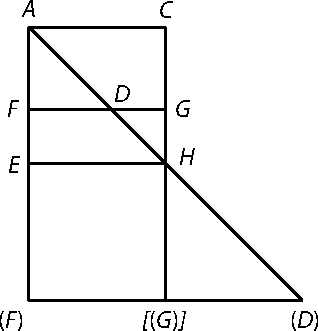
\includegraphics[width=0.36\textwidth]{%
gesamttex/edit_VIII,3/images/LH_37_05_094-095_d_1_094r.pdf%
}%
\hfill\hfill\hfill\hfill\hfill\hfill%
\protect\raisebox{0.3em}{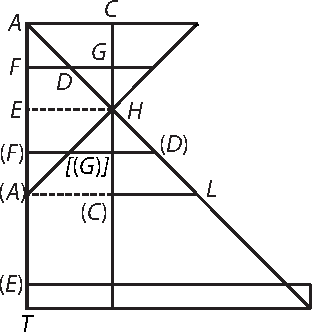
\includegraphics[width=0.36\textwidth]{%
gesamttex/edit_VIII,3/images/LH_35_09_16_016_d_016r.pdf%
}}
\hfill\hfill\hfill\hfill%
} 
\vspace{0.5em}
\centerline{%
\hspace*{5mm}
\hfill
\lbrack\textit{Fig.~1a, L%
}\rbrack \hspace*{35mm}
\lbrack\textit{Fig.~1b, erg.\ Hrsg.\ aus N.~\ref{41169}}\rbrack
\hfill%
}
% \newpage%
\vspace{1.5em}
%
\pstart
\edtext{}{\lemma{\hspace*{1,6mm}% % TRICK, Anmk. zur Figur
\lbrack\textit{Fig.~1a}\rbrack, \lbrack\textit{Fig.~1b}\rbrack%
}\killnumber%
\Cfootnote{Leibniz hat in beiden Diagrammen den Buchstaben \textit{G} an je zwei verschiedene Punkte vergeben; die Bezeichnung des zweiten Punktes ändert Hrsg.}}
%
In \edtext{figura \ldots}{%
\lemma{In figura \ldots}%
\Cfootnote{%
Die Punkte bei \glqq In figura \ldots\grqq\ dienten wohl als Platzhalter für eine später zu ergänzende Figur. Tatsächlich hat Leibniz \lbrack\textit{Fig.~1a}\rbrack\ erst in der Folge gezeichnet, nämlich neben dem Text auf S.~\refpassage{37_05_094-095_7a}{37_05_094-095_7b}. Mit sehr hoher Wahrscheinlichkeit orientierte er sich beim Schreiben an der bestehenden \lbrack\textit{Fig.~1}\rbrack\ von N.~\ref{41169}, die deshalb hier als \lbrack\textit{Fig.~1b}\rbrack\ ergänzt wird. Davon zeugen die genaue Übereinstimmung der Punktebezeichnungen im Text mit \lbrack\textit{Fig.~1b}\rbrack\ und die Abweichungen von \lbrack\textit{Fig.~1a}\rbrack. Siehe die Vorbemerkung zu N.~\ref{comp_non_fidendum}.}}
%
\edtext{ponatur tempus \textit{AE}, celeritas \textit{AC}, vel \textit{FG} vel \textit{EH}, qua}{%
\lemma{ponatur}%
\Bfootnote{\textit{(1)}~grave ascendere %
\textit{(2)}~tempus \textit{AE}, celeritas \textit{AC}, %
\textbar\ vel \textit{FG} vel \textit{EH}, \textit{erg.}~\textbar\ qua~\textit{L}}} %
%
grave\protect\index{Sachverzeichnis}{grave} moveatur sursum; et quovis momento ascensus ut \textit{F}, 
%
\edtext{sit}{\lemma{}\Bfootnote{sit \textit{erg.~L}}} 
%
celeritas \textit{FD} 
%
\edtext{(ordinata trianguli \textit{AEH})}{\lemma{}\Bfootnote{(ordinata trianguli \textit{AEH}) \textit{erg.~L}}} 
%
qua grave moveatur
%
\edtext{deorsum; his positis}{%
\lemma{deorsum}%
\Bfootnote{\textit{(1)}~, \textit{(2)}~; his positis~\textit{L}}} 
%
erit \textit{DG} celeritas residua ascensus, quae in \textit{H} evanescet. 
%
Sequenti igitur tempore \textit{E}(\textit{A}) si ambos motus ponamus continuari, motumque sursum 
%
repraesentari rectangulo
%
\textit{HE}(\textit{A})(\textit{C}), deorsum trapezio \textit{E}(\textit{A})\textit{LH} 
%
((quod est continuatio trianguli \textit{AEH}, ut inde fiat triangulum \textit{A}(\textit{A})\textit{L})) 
%
patet motum deorsum praevalere, et
%
repraesentari triangulo
%
\textit{H}(\textit{C})\textit{L}, gravi scilicet in momento \textit{E} rursum descendere 
%
\edtext{incipiente, et triangulum}{\lemma{incipiente,}\Bfootnote{\textit{(1)}~eadem celeritate \textit{(2)}~et triangulum~\textit{L}}}
%
\textit{H}(\textit{C})\textit{L} per omnia simile esse et aequale triangulo \textit{AEH} 
%
\edtext{et grave in (\textit{A}) rursus attingere horizontalem ex qua momento \textit{A} sursum ascenderat.}{%
\lemma{}%
\Bfootnote{et grave \lbrack...\rbrack\ ascenderat. \textit{erg.~L}}} 
%
Et proinde, hoc modo non potest notari error practicus%
\protect\index{Sachverzeichnis}{error practicus} in hac Hypothesi,
%
sed si \edtext{fingeremus aliam}{\lemma{fingeremus}%
\Bfootnote{\textit{(1)}~grave in momento (\textit{A}) quo rursus pavimentum %
attingit ab eo perfecto elastro reflecti, ita ut tempore %
\textit{(a)}~(\textit{A})(\textit{E}) \textit{(b)}~(\textit{A})(\textit{E}) aequali ipsi \textit{AE} %
\textit{(2)}~lineam \textit{(3)}~aliam~\textit{L}}}
 %
esse proportionem accelerationis,%
\protect\index{Sachverzeichnis}{proportio accelerationis} non scilicet uniformem, ac proinde lineam 
%
\edtext{\textit{AD}\lbrack(\textit{D})\rbrack}{%
\lemma{}%
\Bfootnote{%
\textit{ADD} %
\textit{L ändert Hrsg.}}}
 %
non esse rectam, sed aliam, verbi gratia parabolicam, vel etiam alterius naturae,
%
\edtext{quemadmodum revera non foret}{\lemma{}%
\Afootnote{\textit{Am Rand}: NB}} 
%
recta, si poneremus impetum quo gravia\protect\index{Sachverzeichnis}{grave} 
%
\edtext{descendunt, non uniformiter}{\lemma{descendunt, non}\Bfootnote{\textit{(1)}~esse \textit{(2)}~uniformiter~\textit{L}}}
%
augeri, sed \edtext{gravia quo magis}{\lemma{}\Bfootnote{gravia \textbar\ quo \textit{erg.}~\textbar\ magis~\textit{L}}} 
%
ad terram\protect\index{Sachverzeichnis}{terra} appropinquant,
%
eo fortius attrahi; tunc ista motuum compositio%
\protect\index{Sachverzeichnis}{compositio motuum} etiam cum experientia%
\protect\index{Sachverzeichnis}{experientia} pugnatura esset.
%
Si enim \edtext{figura curvilinea}{\lemma{figura}\Bfootnote{curvilinea \textit{erg.~L}}} \textit{H}(\textit{C})\textit{L} 
%
minor esset quam \edtext{figura curvilinea}{\lemma{}\Bfootnote{figura curvilinea \textit{erg.~L}}} \textit{AEH},
%
utique grave minore tempore terram rursus descendendo \edlabel{37_05_094-095_7a}attingeret quam qua ascendit, abstrahendo licet animum, 
%
ab omni resistentia aeris\protect\index{Sachverzeichnis}{resistentia aeris} aut simili impedimento, 
%
foretque adeo effectus suae causae inaequalis.%
\protect\index{Sachverzeichnis}{effectus suae causae inaequalis} 
%
\edtext{Itaque doctrina}{\lemma{}\Bfootnote{Itaque \textbar\ ista \textit{gestr.}~\textbar\ doctrina~\textit{L}}} 
%
de Motuum compositionibus%
\protect\index{Sachverzeichnis}{doctrina de compositionibus motuum} non est admittenda, nisi quatenus 
%
\edtext{cum summis potentiarum\protect\index{Sachverzeichnis}{summa potentiarum}}{\lemma{cum}%
\Bfootnote{\textit{(1)}~potentiis \textit{(2)}~summis potentiarum~\textit{L}}}
%
conciliari potest; alioqui figmenti potius quam realitatis
%
\edtext{loco habenda erit, si}{%
\lemma{loco}%
\Bfootnote{\textit{(1)}~erit \textit{(2)}~habenda erit %
\textit{(a)}~. Hinc et in n \textit{(b)}~. Et quand \textit{(c)}~, si~\textit{L}}} 
%
ab ipsa natura non praeitur nobis 
%
\edtext{via. Unde}{%
\lemma{via.}%
\Bfootnote{%
\textit{(1)}~Ut %
\textit{(2)}~Unde~\textit{L}}}
%
non succedit \edtext{simpliciter}{\lemma{}\Bfootnote{simpliciter \textit{erg.~L}}}
%
compositio motuum%
\protect\index{Sachverzeichnis}{compositio motuum} in ictibus 
%
\edtext{obliquis,\protect\index{Sachverzeichnis}{ictus obliquus} nisi\edlabel{37_05_094-095_7b}}{\lemma{obliquis,}%
\Bfootnote{\textit{(1)}~nisi \textit{(2)}~si \textit{(3)}~nisi~\textit{L}}} 
%
quando angulus quem duae directiones motuum compositorum faciunt, est rectus. 
%
Quemadmodum \edtext{in separata scheda}{%
\lemma{in separata scheda}%
\Cfootnote{Gemeint ist die Aufzeichnung N.~\ref{41167}; siehe bes.\ die Randanmerkung zu S.~\refpassage{35_09_16_017_3a}{35_09_16_017_3b}.}} 
%
\edtext{ostendi, et modum etiam}{\lemma{ostendi,}%
\Bfootnote{\textit{(1)}~modumque etia \textit{(2)}~et modum etiam~\textit{L}}} 
%
explicui, quomodo sit procedendum, quando ab uno corpore duo impelluntur 
%
\edtext{simul, eodem modo,}{\lemma{simul}%
\Bfootnote{\textit{(1)}~eodem modo \textit{(2)}~, eodem modo,~\textit{L}}}
%
linea ad utrumque obliqua et inter ipsa media, ex 
%
\edlabel{37_05_094-095_8a}%
\edtext{}{% 
{\xxref%
{37_05_094-095_8a}{37_05_094-095_8b}}%
\lemma{regula \lbrack...\rbrack\ alternorum}%
\Cfootnote{%
Zur Formulierung der \glqq regula alternativorum\grqq\ siehe \textsc{G.\,W.\,Leibniz}, \cite{01098}\glqq Demonstratio geometrica regulae apud Staticos receptae\grqq, in \cite{01023}\textit{AE}, November 1685, S.~501\textendash505, hier S.~503\textendash505. Das Stück erscheint in einem späteren Band der Reihe.%
}}%
regula scilicet concursus Electivi
%
\edtext{alternorum.\protect\index{Sachverzeichnis}{regula concursus electivi alternorum}\edlabel{37_05_094-095_8b} Porro}{\lemma{}%
\Bfootnote{alternorum \textbar\ et \textit{erg. u. gestr.}~\textbar\ . Porro~\textit{L}}} 
%
si non fingatur a nobis compositio duorum motuum, sed ab ipsa natura exhibeatur, 
%
\edtext{ut si corpus}{\lemma{ut si}\Bfootnote{\textit{(1)}~navis feratur \textit{(2)}~corpus~\textit{L}}}
%
aliquod, verbi gratia navis\protect\index{Sachverzeichnis}{navis} cum corpore aliquo imposito feratur certo aliquo motu, et corpus 
%
impositum tamen simul in navi\protect\index{Sachverzeichnis}{navis} feratur motu 
%
\edtext{contrario, revera}{\lemma{contrario,}%
\Bfootnote{\textit{(1)}~dico motum corporis in navi quidem posse suos habere effectus, %
sed quatenus non motu navis conjunctus spectatur, corpus hoc habendum pro nullo, %
perinde ac si quiesceret. Itaque si navis impingat in aliud corpus, %
\textit{(2)}~revera~\textit{L}}}
%
duplex erit potentia. Quaeritur autem si navis\protect\index{Sachverzeichnis}{navis} in aliud corpus impingat, an vis
%
impactus\protect\index{Sachverzeichnis}{vis impactus} eadem sit, sive corpus in navi
%
positum quiescat, sive peculiari in navi motu cieatur, et dico eandem esse
%
(\phantom)\hspace*{-1.2mm}nisi forte eo momento non cohaereat navi\protect\index{Sachverzeichnis}{navis} 
%
sed in aere\protect\index{Sachverzeichnis}{aer} saltum exerceat\phantom(\hspace*{-1.2mm}). Causa est, 
%
\edtext{quod si navis\protect\index{Sachverzeichnis}{navis}}{\lemma{quod}%
\Bfootnote{\textit{(1)}~corpus illud \textit{(2)}~si navis~\textit{L}}} 
%
ex impactu\protect\index{Sachverzeichnis}{impactus} repellitur, corpus in navi simul etiam repelletur, et praeter suum 
%
motum hunc accipiet novum. 
\pend
%
\pstart
Itaque corpori cuilibet tribuenda erit potentia motrix\lbrack:\rbrack\protect\index{Sachverzeichnis}{potentia motrix}
%
\edtext{primum}{\lemma{}\Bfootnote{primum \textit{erg.~L}}}
%
secundum mutationem
%
\edtext{qua a corporis alterius}{\lemma{qua a}\Bfootnote{\textit{(1)}~vicini corporis %
\textit{(2)}~corporis alterius~\textit{L}}} 
%
immediato contactu\protect\index{Sachverzeichnis}{contactus immediatus} recedit, si quidem causa recessus%
\protect\index{Sachverzeichnis}{causa recessus} sit in ipso,
%
\edtext{aut in quantum}{\lemma{aut}\Bfootnote{\textit{(1)}~qua \textit{(2)}~in quantum~\textit{L}}}
%
est in ipso; deinde \edtext{etiam}{%
\lemma{}%
\Bfootnote{%
etiam %
\textit{erg.~L}}}
%
si ut pars consideretur alterius corporis, et cum eo motum habeat communem, praeter eum quem habet in ipso, 
%
ut sanguis\protect\index{Sachverzeichnis}{sanguis} cum homine\protect\index{Sachverzeichnis}{homo}, 
%
pila\protect\index{Sachverzeichnis}{pila} in navi\protect\index{Sachverzeichnis}{navis} decurrens,
%
cum navi\protect\index{Sachverzeichnis}{navis}, \edtext{tunc}{%
\lemma{}%
\Bfootnote{%
tunc %
\textit{erg.~L}}}
%
eatenus etiam ipsi tribuenda est vis motrix%
\protect\index{Sachverzeichnis}{vis motrix}
%
\edtext{in quantum ejus corporis pars est}{\lemma{}\Bfootnote{in quantum ejus corporis pars est \textit{erg.~L}}}. Et 
%
\edtext{proinde corpori}{%
\lemma{proinde}%
\Bfootnote{\textit{(1)}~corpus habet \textit{(2)}~corpori~\textit{L}}}
%
non tribuendus est tantum motus qui agnoscitur contactus immediati%
\protect\index{Sachverzeichnis}{contactus immediatus} mutatione, 
%
sed etiam communis; nec tantum tribuendus est ei motus in linea ex motibus illis compositis resultante, 
%
ita enim corpori forte tribuenda esset 
%
\edtext{quies,\protect\index{Sachverzeichnis}{quies} quando forte duos diversos motus contrarios aequales%
\protect\index{Sachverzeichnis}{motus contrarii aequales} habet, cum tamen duplici}{%
\lemma{quies,}%
\Bfootnote{\textit{(1)}~cum tamen duos diversos motus contrarios habeat, duplicique %
\textit{(2)}~quando \lbrack...\rbrack\ duplici~\textit{L}}} 
%
modo potentiam\protect\index{Sachverzeichnis}{potentia} exercere possit, sed tribuenda ei utraque 
%
potentia\protect\index{Sachverzeichnis}{potentia} est separatim, quia utriusque
%
 mutationis ratio in ipso est vel pro toto, vel saltem pro parte.
\pend
%
\pstart
Caeterum ex his
%
quae de cautionibus circa compositionem Motuum%
\protect\index{Sachverzeichnis}{compositio motuum} necessariis diximus, consequens est, ut corrigantur, 
 %
\edtext{qui Galileanam doctrinam\protect\index{Sachverzeichnis}{doctrina Galileana} de % %C-FN
\edtext{Motu gravium}{\lemma{Motu}%
\Bfootnote{\textit{(1)}~projectorum \textit{(2)}~gravium~\textit{L}}}
%
oblique vel horizontaliter projectorum,%
\protect\index{Sachverzeichnis}{motus gravium projectorum} et
%
\edtext{lineam compositam}{%
\lemma{lineam}%
\Bfootnote{%
\textit{(1)}~ex mixtura motu %
\textit{(2)}~compositam~\textit{L}}}
%
describentium, demonstrant simplici horum Motuum, violenti%
\protect\index{Sachverzeichnis}{motus violentus} et naturalis,%
\protect\index{Sachverzeichnis}{motus naturalis} %
\lbrack94~v\textsuperscript{o}\rbrack\ compositione.}{%
\lemma{qui Galileanam \lbrack...\rbrack\ compositione}%
\Cfootnote{%
\protect\index{Namensregister}{\textso{Galilei} (Galilaeus, Galileus), Galileo 1564\textendash1642}\textsc{G.~Galilei}, %
\cite{00050}\title{Discorsi}, Giornata Quarta, Leiden 1638, S.~236\textendash288 %	%Leiden
(\cite{00048}\textit{GO} VIII, S.~268\textendash313). %
Leibnizens Kritik richtet sich wahrscheinlich u.a.\ gegen \protect\index{Namensregister}{\textso{Wallis} (Wallisius), John 1616\textendash1703}Wallis' Vorgehen hinsichtlich des \glqq ascensus retardatus\grqq, in \cite{00301}\textit{Mechanica}, London 1670\textendash1671, Pars~III, Cap.~X, Prop.~III, S.~648\textendash650 (\cite{01008}\textit{WO} I, S.~994f.), und der Wurfbahn, \cite{00301}a.a.O., Prop.~VIII, S.~658f. (\cite{01008}\textit{WO} I, S.~1001).}}
%
\pend
%
\pstart
Etsi enim hoc per accidens hic eveniat in casu accelerationis uniformis,%
\protect\index{Sachverzeichnis}{acceleratio uniformis} si tamen acceleratio esset %
%
\edtext{difformis\protect\index{Sachverzeichnis}{acceleratio difformis} quo casu}{\lemma{difformis}%
\Bfootnote{\textit{(1)}~aliaque \textit{(2)}~quo casu~\textit{L}}} et linea
%
\edtext{\textit{AD}\lbrack(\textit{D})\rbrack}{%
\lemma{}% 
\Bfootnote{\textit{ADD} \textit{erg.~L, ändert Hrsg.}}} 
%
velocitat\textlangle um\textrangle\ (seu incrementorum spatii)%
\protect\index{Sachverzeichnis}{incrementum spatii} ad tempus % 
% 
\edtext{\textit{AE}}{\lemma{}% 
\Bfootnote{\textit{AE} \textit{erg.~L}}} applicatarum, foret alia quam recta% 
% 
\edtext{, tunc}{\lemma{, tunc}% 
\Bfootnote{\textit{erg.~L}}} non succeder\textlangle et\textrangle\
%
hypothesis compositionis,\protect\index{Sachverzeichnis}{hypothesis compositionis motuum} ut jam notavimus.
%
\edtext{Itaque recte aliquis apud Wallisium\protect\index{Namensregister}{\textso{Wallis} (Wallisius), John 1616\textendash1703} %
(quem ipse tamen non nominat) invito licet Wallisio\protect\index{Namensregister}{\textso{Wallis} (Wallisius), John 1616\textendash1703} motuum compositioni%
\protect\index{Sachverzeichnis}{compositio motuum} non putat fidendum.}%
{\lemma{Itaque \lbrack...\rbrack\ fidendum}\Cfootnote{%
\cite{00301}a.a.O., Pars~III, Cap.~XIII, Scholium zu Prop.~II, S.~693 (\cite{01008}\textit{WO} I, S.~1022).
}}
%
\edlabel{37_05_094-095_1a}%
\edtext{}{% C-Footnote – "Et Tartalea... componebat"
{\xxref%
{37_05_094-095_1a}{37_05_094-095_1b}}%
\lemma{Et Tartalea \lbrack...\rbrack\ componebat}%
\Cfootnote{%
\protect\index{Namensregister}{\textso{Tartaglia} (Tartalea), Niccol{\`o} 1499 o. 1500\textendash1557}%
\textsc{N.~Tartaglia}, \cite{02017}\textit{Nova Scientia} (2.~Ausgabe), Venedig 1550, Libro~I, Prop.~V, Bl.~7~r\textsuperscript{o}.%
}}%
\edtext{Et Tartalea\protect\index{Namensregister}{\textso{Tartaglia} (Tartalea), Niccol{\`o} 1499 o. 1500\textendash1557}}{%
\lemma{Et}%
\Bfootnote{\textit{(1)}~Nicol. \textit{(2)}~quo \textit{(3)}~Tartagli \textit{(4)}~Tartalea~\textit{L}}} %
quoque contra alium non absurde %
\edtext{disputabat, qui}{\lemma{disputabat,}% 
\Bfootnote{\textit{(1)}~quia \textit{(2)}~qui~\textit{L}}} 
duos motus naturalem%
\protect\index{Sachverzeichnis}{motus naturalis} et violentum%
\protect\index{Sachverzeichnis}{motus violentus} componebat.%
\edlabel{37_05_094-095_1b}
%
Forte enim simile quid in mente ipsi fuit. 
%
Non ergo putandum est motum violentum%
\protect\index{Sachverzeichnis}{motus violentus} componi cum naturali, et videri tantum destrui, quod % 
% 
\edtext{naturalis\protect\index{Sachverzeichnis}{motus naturalis} fiat semper valentior, utroque revera %
manente\lbrack;\rbrack\ sed potius revera destrui in gravi\protect\index{Sachverzeichnis}{grave} sive potius amitti, dum in Aetherem\protect\index{Sachverzeichnis}{aether}}{\lemma{naturalis}% 
\Bfootnote{\textit{(1)}~vi \textit{(2)}~fiat %
\textit{(a)}~deterior \textit{(b)}~semper valentior, %
\textit{(aa)}~sed \textit{(bb)}~utroque revera manente, sed potius revera destrui in %
\textit{(aaa)}~corpore  atque \textit{(bbb)}~gravi sive potius amitti, \textit{(aaaa)}~contr \textit{(bbbb)}~dum in %
\textit{(aaaaa)}~corpora \textit{(bbbbb)}~Aetherem~\textit{L}}}
%
occurrentem et ascendenti obnitentem paulatim transfertur.
\pend
%
\vspace{1.0em} %%%%%%%%% Diagramm 2
\centerline{%
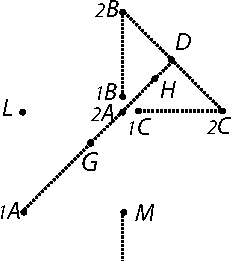
\includegraphics[width=0.25\textwidth]{%
gesamttex/edit_VIII,3/images/LH_37_05_094-095_d_2_094v.pdf%
}} 
\vspace{0.5em}
\centerline{%
\lbrack\textit{Fig.~2}\rbrack%
}
% \newpage%
\vspace{1em}
%
\pstart
%
\hspace{1mm}\hspace{-1mm}% Trick, weil \edlabel nicht zu \par-Beginn sein darf
\edlabel{37_05_094-095_10a}% %edlabel für Datierung
Denique ut clarius appareat quam non sit fidendum compositioni motuum%
\protect\index{Sachverzeichnis}{compositio motuum} % 
% 
\edtext{ostendam succedere consequentias inde deductas, cum angulus %
directionum diversarum inter se compositarum est rectus,%
\protect\index{Sachverzeichnis}{angulus rectus} non vero cum est obliquus%
\protect\index{Sachverzeichnis}{angulus obliquus}}{\lemma{}% 
\Bfootnote{ostendam succedere \lbrack...\rbrack\ est obliquus \textit{erg.~L}}}. % 
% 
\edtext{Sit rectangulum}{\lemma{Sit}% 
\Bfootnote{\textit{(1)}~quadratum \textit{(2)}~rectangulum~\textit{L}}}
%
\textit{L.{\scriptsize1}A.M.{\scriptsize2}A}. et recta \textit{L{\scriptsize2}A} producatur in \textit{{\scriptsize1}C{\scriptsize2}C},
%
recta vero \textit{M{\scriptsize2}A}
%
\edtext{in \textit{{\scriptsize1}B{\scriptsize2}B}, sitque \textit{{\scriptsize2}A{\scriptsize2}B} %
(vel \textit{{\scriptsize1}B{\scriptsize2}B}) aequalis}{%
\lemma{in \textit{{\scriptsize1}B{\scriptsize2}B},}%
\Bfootnote{%
\textit{(1)}~sintque \textit{{\scriptsize2}A{\scriptsize2}B} (vel \textit{{\scriptsize1}B{\scriptsize2}B}) et %
\textit{(2)}~sitque \textit{{\scriptsize2}A{\scriptsize2}B} (vel \textit{{\scriptsize1}B{\scriptsize2}B}) aequalis~\textit{L}}}
%
 ipsi \textit{M{\scriptsize2}A}, et recta
%
\textit{{\scriptsize2}A{\scriptsize2}C} (seu \textit{{\scriptsize1}C{\scriptsize2}C}) aequalis ipsi \textit{L{\scriptsize2}A}
%
(pono enim \textit{{\scriptsize2}A}, \textit{{\scriptsize1}B}, \textit{{\scriptsize1}C}, quasi in unum punctum coincidere). 
%
His positis si sint tria corpora aequalia \textit{A}, \textit{B}, \textit{C}, et \textit{A} veniens ex \textit{{\scriptsize1}A}  
%
in \textit{{\scriptsize2}A}, ibique % 
% 
\edtext{impingens simul in duo}{\lemma{impingens}% 
\Bfootnote{\textit{(1)}~in duo \textit{(2)}~simul in duo~\textit{L}}}
%
\textit{B} et \textit{C} quiescentia in \textit{{\scriptsize1}B}, \textit{{\scriptsize1}C}, tunc % 
% 
si \textit{A} habuit
% 
\edtext{celeritatem%
\protect\index{Sachverzeichnis}{celeritas} et directionem%
\protect\index{Sachverzeichnis}{directio} \textit{{\scriptsize1}A{\scriptsize2}A}, \textit{A} quidem}{%
\lemma{celeritatem}% 
\Bfootnote{\textit{(1)}~ut \textit{{\scriptsize1}A{\scriptsize2}A}, \textit{(2)}~et directionem \textit{{\scriptsize1}A{\scriptsize2}A}, \textit{(a)}~habebi\textlangle t\textrangle\ \textit{(b)}~\textit{A} quidem~\textit{L}}}
%
quiescet post impactum in \textit{{\scriptsize2}A}, at \textit{B} accipiet celeritatem et directionem
%
\textit{{\scriptsize1}B{\scriptsize2}B} et \textit{C} accipiet celeritatem atque directionem % 
% 
\edtext{\textit{{\scriptsize1}C{\scriptsize2}C}, ita ut \textit{A},}{%
\lemma{\textit{{\scriptsize1}C{\scriptsize2}C},}% 
\Bfootnote{\textit{(1)}~et haec quidem directio motuum \textit{(2)}~ita ut \textit{A},~\textit{L}}}
%
duas habuisse ponatur celeritates atque directiones, unam \textit{{\scriptsize1}AL}, quam tribuit corpori \textit{B}, quod solum ipsi % 
% 
obstat, alteram \textit{{\scriptsize1}AM}, quam tribuit corpori % 
% 
\edtext{obstanti \textit{C}. Id vero}{\lemma{obstanti \textit{C}.}% 
\Bfootnote{\textit{(1)}~Atque hoc quidem modo pulchre procedit compositio Motuu \textit{(2)}~Id vero~\textit{L}}}
%
pulcherrime consentit cum aggregato virium,\protect\index{Sachverzeichnis}{aggregatum virium} tam ante %
quam post impactum\protect\index{Sachverzeichnis}{impactus}, 
%
nam non tantum eadem servatur directio%
\protect\index{Sachverzeichnis}{directio centri gravitatis} et celeritas centri gravitatis%
\protect\index{Sachverzeichnis}{celeritas centri gravitatis} 
%
trium corporum communis\protect\index{Sachverzeichnis}{centrum gravitatis commune trium corporum} %
ante et post impactum\protect\index{Sachverzeichnis}{impactus}, sed et eadem potentia %
absoluta\protect\index{Sachverzeichnis}{potentia absoluta} quae aestimatur quadrato celeritatis ducto in corpus.%
\protect\index{Sachverzeichnis}{quadratum celeritatis ductum in corpus} % 
% 
\edtext{Nam cum}{\lemma{Nam}% 
\Bfootnote{\textit{(1)}~quadratum \textit{(2)}~cum~\textit{L}}}
%
corpora tria sint aequalia, neglig\textlangle i\textrangle\ potest molis eorum consideratio, et sufficit considerari quadrata linearum, jam % 
% 
\edtext{ob angulum \textit{B.{\scriptsize2}A.C} rectum,}{\lemma{}% 
\Bfootnote{ob angulum \textit{B.{\scriptsize2}A.C} rectum, \textit{erg.~L}}} 
%
quadratum ipsius \textit{{\scriptsize1}A{\scriptsize2}A} celeritatis%
\protect\index{Sachverzeichnis}{quadratum celeritatis}
%
ante impactum\protect\index{Sachverzeichnis}{impactus}, 
%
\edtext{aequatur quadratis ipsarum \textit{{\scriptsize1}B{\scriptsize2}B}}{%
\lemma{aequatur}%
\Bfootnote{%
\textit{(1)}~quadrato \textit{{\scriptsize1}B{\scriptsize2}B} %
\textit{(2)}~quadratis ipsarum \textit{{\scriptsize1}B{\scriptsize2}B}~\textit{L}}}
% 
(hoc est \textit{{\scriptsize1}AL}) et \textit{{\scriptsize1}C{\scriptsize2}C} (hoc est \textit{{\scriptsize1}AM})
%
celeritatum post impactum\protect\index{Sachverzeichnis}{impactus}, atque ita res pulchre procedit sane, 
%
si angulus \textit{BAC} sit 
%
\edtext{rectus, ut posuimus}{%
\lemma{rectus, ut}%
\Bfootnote{%
\textit{(1)}~huc %
\textit{(2)}~posuimus~\textit{L}}}
%
huc usque.
\pend 
%
\vspace{1.0em} %%%%%%%%% Diagramm 3
\centerline{%
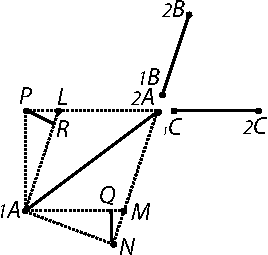
\includegraphics[width=.275\textwidth]{%
gesamttex/edit_VIII,3/images/LH_37_05_094-095_d_3_094v.pdf%
}} 
\vspace{0.5em}
\centerline{%
\lbrack\textit{Fig.~3}\rbrack%
}
% \newpage%
\vspace{1em}
%
\pstart
Sed
%
nunc videamus quid fiat si sit obliquus;%
\protect\index{Sachverzeichnis}{angulus obliquus} 
%
seu si caeteris positis ut ante, parallelogrammum 
%
\textit{L{\scriptsize1}AM{\scriptsize2}A} non sit rectangulum,%
\protect\index{Sachverzeichnis}{parallelogrammum rectangulum} sed % 
% 
\edtext{obliquum.\protect\index{Sachverzeichnis}{parallelogrammum obliquum} Si igitur}{\lemma{obliquum.}% 
\Bfootnote{\textit{(1)}~Non poterit \textit{(2)}~Si igitur~\textit{L}}} 
%
corpus \textit{A}, habens celeritatem%
\protect\index{Sachverzeichnis}{celeritas} et directionem%
\protect\index{Sachverzeichnis}{directio} \textit{{\scriptsize1}A{\scriptsize2}A} det corpori \textit{B} celeritatem % 
% 
\edtext{et directionem \textit{{\scriptsize1}B}\lbrack\textit{{\scriptsize2}B}\rbrack, parallelam}{%
\lemma{et directionem}% 
\Bfootnote{%
\textbar\ \textit{{\scriptsize1}B{\scriptsize1}C} \textit{ändert Hrsg.}~\textbar\ %
, \textit{(1)}~aequalem \textit{(2)}~parallelam~\textit{L}}}
%
ipsi \textit{{\scriptsize1}AL}, corpori vero \textit{C} directionem et celeritatem
%
\textit{{\scriptsize1}C{\scriptsize2}C} parallelam ipsi \textit{{\scriptsize1}AM}; 
%
tunc nego fieri posse ut \textit{{\scriptsize1}B{\scriptsize2}B} sit aequalis ipsi 
%
\textit{{\scriptsize1}AL}, et \textit{{\scriptsize1}C{\scriptsize2}C} ipsi \textit{{\scriptsize1}AM} 
%
quemadmodum videbitur illis, qui motuum compositionem%
\protect\index{Sachverzeichnis}{compositio motuum} sequentur, quasi scilicet corpus 
%
\textit{A} habere ponatur duplicem celeritatem et directionem, % 
% 
\edtext{unam, \textit{{\scriptsize1}AL},}{\lemma{unam,}% 
\Bfootnote{\textit{(1)}~\textit{{\scriptsize1}A{\scriptsize1}L} \textit{(2)}~\textit{{\scriptsize1}AL},~\textit{L}}}
%
quam det corpori \textit{B}, alteram \textit{{\scriptsize1}AM} quam det corpori \textit{C}. 
%
Nego enim hanc compositionem motuum corporis \textit{A}, etsi imaginationi%
\protect\index{Sachverzeichnis}{imaginatio} satisfaciat, et Geometricis % 
% 
\edtext{considerationibus,\protect\index{Sachverzeichnis}{consideratio geometrica} etiam realitati\protect\index{Sachverzeichnis}{realitas}}{\lemma{considerationibus, etiam}% 
\Bfootnote{\textit{(1)}~realitatibus \textit{(2)}~realitati~\textit{L}}}  
%
et physicis effectibus\protect\index{Sachverzeichnis}{effectus physicus} posse satisfacere. Ex % 
% 
\edtext{quo etiam apparet,}{\lemma{quo etiam}% 
\Bfootnote{\textit{(1)}~apparent \textit{(2)}~apparet,~\textit{L}}} 
%
quantum inter Geometrica seu incompleta,%
\protect\index{Sachverzeichnis}{Geometrica seu incompleta} 
%
et realia sive \protect{\pgrk{f}ysica}%
\protect\index{Sachverzeichnis}{realia sive physica} intersit. 
%
\edtext{Nam non}{%
\lemma{Nam}%
\Bfootnote{%
\textit{(1)}~si %
\textit{(2)}~non~\textit{L}}}
%
ut in angulo recto%
\protect\index{Sachverzeichnis}{angulus rectus} \textit{LAM} paulo ante successerat, ita
%
nunc in obliquo%
\protect\index{Sachverzeichnis}{angulus obliquus} succedere potest, ut % 
% 
\edtext{quadrata ipsarum \textit{{\scriptsize1}AL}, (\phantom)\hspace*{-1.2mm}seu}{\lemma{quadrata}% 
\Bfootnote{\textit{(1)}~\textit{{\scriptsize1}AL} et \textit{{\scriptsize1}A} %
\textit{(2)}~ipsarum \textit{{\scriptsize1}AL}, \textit{(a)}~et \textit{{\scriptsize1}AM} (\phantom)\hspace*{-1.2mm}seu %
\textit{(b)}~(\phantom)\hspace*{-1.2mm}seu~\textit{L}}} 
%
\textit{{\scriptsize1}B{\scriptsize2}B}\phantom(\hspace*{-1.2mm}) et \textit{{\scriptsize1}AM} 
%
(seu \textit{{\scriptsize1}C{\scriptsize2}C}) simul aequentur quadrato ipsius
%
\textit{{\scriptsize1}A{\scriptsize2}A}, quod tamen fieri deberet, % 
% 
\edtext{quia ante}{\lemma{quia}% 
\Bfootnote{\textit{(1)}~post \textit{(2)}~ante~\textit{L}}} 
%
impactum erat celeritas \textit{{\scriptsize1}A{\scriptsize2}A}, post impactum 
%
celeritates \textit{{\scriptsize1}B{\scriptsize2}B}, et \textit{{\scriptsize1}C{\scriptsize2}C}. Quid ergo dicemus in hoc % 
% 
\edtext{casu anguli obliqui}{\lemma{casu}% 
\Bfootnote{\textit{(1)}~impactus obliqui \textit{(2)}~anguli obliqui~\textit{L}}},
%
eritne solutio supra scientiae nostrae vires? Non utique; etsi % 
% 
\edtext{putem eam}{\lemma{putem}% 
\Bfootnote{\textit{(1)}~solutionem \textit{(2)}~eam~\textit{L}}} 
%
non fore cujus vis. Sic ergo procedemus, utendo compositione anguli recti, 
%
cujus realitatem\protect\index{Sachverzeichnis}{realitas} supra stabilivimus %
ad solvendam difficultatem obliqui. % 
% 
\edtext{\textit{BM} producatur (si opus)}{\lemma{\textit{BM} producatur}% 
\Bfootnote{%
\textit{(1)}~usq \textit{(2)}~ubi \textit{(3)}~(si opus)~\textit{L}}}  
%
in \textit{N} ubi ei ad angulos rectos occurrat \textit{{\scriptsize1}AN} et \textit{CL} producatur (si opus) in \textit{P} 
%
ubi ei ad angulos rectos occurrat. Utique manifestum est ex superioribus 
%
si sola adessent corpora \textit{A} et \textit{B}, corpus \textit{A}, % 
\edtext{celeritate et}{\lemma{celeritate}% 
\Bfootnote{et \textit{erg.~L}}} 
%
directione \textit{{\scriptsize1}A{\scriptsize2}A} incurrens corpori \textit{B} quiescenti % 
% 
\edtext{in \textit{{\scriptsize1}B} perinde}{\lemma{in \textit{{\scriptsize1}B}}% 
\Bfootnote{\textit{(1)}~daturum ipsi esse \textit{(2)}~perinde~\textit{L}}}
%
ac si haberet celeritates atque directiones 
%
\textit{{\scriptsize1}AN}, et \textit{N{\scriptsize2}A}, daturum ipsi \textit{B}
%
celeritatem%
\protect\index{Sachverzeichnis}{celeritas} atque directionem%
\protect\index{Sachverzeichnis}{directio} \textit{{\scriptsize1}B{\scriptsize2}B} aequalem ipsi
%
\textit{N{\scriptsize2}A}; et similite\textlangle r\textrangle\ % 
% 
\edtext{corpus \textit{A}, celeritate et directione \textit{{\scriptsize1}A{\scriptsize2}A}}{\lemma{corpus \textit{A},}% 
\Bfootnote{\textit{(1)}~directione \textit{{\scriptsize1}A{\scriptsize2}A} %
\textit{(2)}~celeritate et directione \textit{{\scriptsize1}A{\scriptsize2}A}~\textit{L}}}
%
(hoc est \textit{{\scriptsize1}AP} et \textit{P{\scriptsize2}A}) incurre\textlangle ns\textrangle\ % 
% 
\edtext{soli}{\lemma{}% 
\Bfootnote{soli \textit{erg.~L}}} % 
% 
\edtext{corpori \textit{C} quiescenti}{\lemma{corpori \textit{C}}% 
\Bfootnote{\textit{(1)}~daturum esse ipsi \textit{(2)}~quiescenti~\textit{L}}} 
%
in \textit{{\scriptsize1}C} daturum esse ipsi \textit{C} celeritatem et directionem \textit{{\scriptsize1}C{\scriptsize2}C} aequalem ipsi \textit{P{\scriptsize2}A}. 
%
Sed nunc cum ambo simul impellantur, \textit{B} et \textit{C} hoc fieri non pot\textlangle est\textrangle\
%
nam quadrata \textit{P{\scriptsize2}A} et \textit{N{\scriptsize2}A} simul majora sunt quadrato \textit{{\scriptsize1}A{\scriptsize2}A}. 
%
An ergo dicemus \textit{{\scriptsize1}B{\scriptsize2}B}, et \textit{{\scriptsize1}C{\scriptsize2}}\textlangle \textit{C},\textrangle\ 
%
sumendas esse tales, ut sit quadr.\ \textit{{\scriptsize1}B{\scriptsize2}B} ad \textit{N{\scriptsize2}A}, et  
%
\textit{{\scriptsize1}C{\scriptsize2}C} ad \textit{P{\scriptsize2}A}, ut quadrata \textit{N{\scriptsize2}A} et  
%
\textit{P{\scriptsize2}A} simul sunt ad quadratum \textit{{\scriptsize1}A{\scriptsize2}A}.  
%
Atque ita omnino dicendum est; si ponamus corpus \textit{A} quiescere post  
%
\edlabel{37_05_094-095_2a}%
\edtext{}{%
{\xxref{37_05_094-095_2a}{37_05_094-095_2b}}%
\lemma{impactum}% 
\Bfootnote{%
\textit{(1)}~seu et h\textlangle\textendash\textrangle\ \textlangle\textendash\textrangle actum centrum gravitatis omnium trium eadem qua ante, pergere celeritate. \textit{(2)}~\lbrack95~r\textsuperscript{o}\rbrack\ Et certe \textit{(3)}~Verum~\textit{L}}}%
%
impactum.\edlabel{37_05_094-095_10b}	
\pend 
%
\vspace{1.0em} %%%%%%%% Diagramme 4-5
\centerline{\hfill%
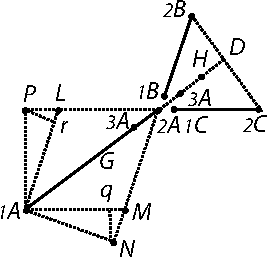
\includegraphics[width=0.275\textwidth]{%
gesamttex/edit_VIII,3/images/LH_37_05_094-095_d_4_094v.pdf%
}%
\hfill%
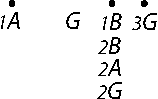
\includegraphics[width=0.175\textwidth]{%
gesamttex/edit_VIII,3/images/LH_37_05_094-095_d_5_094v.pdf%
}\hfill} % 
\vspace{0.5em} %%%%%%%%% 
\hfill\centerline{%
\lbrack\textit{Fig.~4}\rbrack \hspace*{45mm}
\lbrack\textit{Fig.~5}\rbrack%
}\hfill
% \newpage%
\vspace{1em}
%
\pstart
\lbrack95~r\textsuperscript{o}\rbrack\ 
Verum\edlabel{37_05_094-095_2b} 
%
res vel ideo videtur adhuc altioris indaginis, % 
% 
\edtext{quia singulos}{\lemma{quia}% 
\Bfootnote{\textit{(1)}~quolibet s \textit{(2)}~singulos~\textit{L}}}  
%
casus spectando corpus \textit{A} non tantum tribuit ipsis \textit{B} % 
% 
\edtext{et \textit{C}, celeritates ut}{\lemma{et \textit{C},}% 
\Bfootnote{\textit{(1)}~potentias ut \textit{(2)}~celeritates ut~\textit{L}}}  
%
\textit{N{\scriptsize2}A}, \textit{P{\scriptsize2}A}, sed et retinet sibi celeritates et directiones illo solo  
%
existente \textit{{\scriptsize1}AN}, hoc solo existente \textit{{\scriptsize1}AP}. Itaque % 
% 
\edtext{in casu concursus}{\lemma{}% 
\Bfootnote{in casu concursus \textit{erg.~L}}} 
%
 in distribuendis viribus corporis \textit{A} non tantum ratio habenda % 
% 
\edtext{est potentiarum\protect\index{Sachverzeichnis}{potentia} quas}{\lemma{est}% 
\Bfootnote{\textit{(1)}~corporis \textit{(2)}~potentiae qu \textit{(3)}~potentiarum quas~\textit{L}}}  
%
corporibus excipientibus 
%
\edtext{tribuit, ut}{%
\lemma{tribuit,}%
\Bfootnote{%
\textit{(1)}~sed %
\textit{(2)}~ut~\textit{L}}}
%
scilicet eae sint proportionales his quas tribueret, si singula sola exciperent, 
%
sed etiam ut ea quae retinet sint similiter proportionalia. Verum hic rursus considerandum 
%
\edtext{est, an eam potentiam\protect\index{Sachverzeichnis}{potentia} quam corpus \textit{A} retinet %
prae ipso \textit{B} nempe celeritatem%
\protect\index{Sachverzeichnis}{celeritas} et directionem%
\protect\index{Sachverzeichnis}{directio} \textit{{\scriptsize1}AN} convertat}{%
\lemma{est,}%
\Bfootnote{%
\textit{(1)}~eam potentiam quam corpus \textit{A} retinet %
\textit{(a)}~ab %
\textit{(b)}~pr %
\textit{(c)}~prae ipso \textit{B} nempe celeritatem et directionem \textit{{\scriptsize1}AN} converti %
\textit{(2)}~an eam \lbrack...\rbrack\ convertat~\textit{L}}}
%
saltem pro parte in impellendum corpus \textit{C}. 
%
Pro parte inquam, quia \textit{{\scriptsize1}AM}, et \textit{{\scriptsize1}AN} non hic ut 
 % 
\edtext{supra}{\lemma{}% 
\Bfootnote{supra \textit{erg.~L}}}  
%
in angulo recto fieret, coincidunt. Itaque ex \textit{N} demittendo \textit{NQ} perpendicularem % 
% 
\edtext{in \textit{{\scriptsize1}AM} pars}{\lemma{}% 
\Bfootnote{in \textit{{\scriptsize1}AM}~\textbar\ saltem \textit{gestr.}~\textbar\ pars~\textit{L}}}  
%
potentiae residuae % 
% 
\edtext{prae corpore \textit{B} retentae}{\lemma{}% 
\Bfootnote{prae corpore \textit{B} retentae \textit{erg.~L}}}  
%
quae erit quadratum % 
% 
\edtext{\textit{{\scriptsize1}AQ}, possit videri adhuc impendi}{%
\lemma{\textit{{\scriptsize1}AQ},}% 
\Bfootnote{\textit{(1)}~impendetur adhuc \textit{(2)}~possit videri adhuc impendi~\textit{L}}} 
%
corpori \textit{C}. Similiter si ex \textit{P} in \textit{{\scriptsize1}AL} demittas perpendicularem \textit{PR}, erit quadr.\ % 
% 
\edtext{\textit{{\scriptsize1}AR} pars}{\lemma{\textit{{\scriptsize1}AR}}% 
\Bfootnote{\textit{(1)}~potentia \textit{(2)}~pars~\textit{L}}} 
%
potentiae ipsius \textit{{\scriptsize1}AP} quam corpus \textit{A} retinet prae corpore \textit{C}. Et ita % 
% 
\edtext{dicendum fore corpus \textit{B} recipere vim quae respondeat}{\lemma{dicendum}% 
\Bfootnote{\textit{(1)}~erit \textit{(2)}~fore corpus %
\textit{(a)}~\textit{C} impe \textit{(b)}~\textit{B} \textit{(aa)}~impelli \textit{(bb)}~recipere vim quae %
\textit{(aaa)}~aequetur \textit{(bbb)}~respondeat~\textit{L}}} 
%
quadratis % 
% 
\edtext{\textit{N{\scriptsize2}A} et \textit{{\scriptsize1}AR},}{\lemma{\textit{N{\scriptsize2}A} et}% 
\Bfootnote{\textit{(1)}~\textit{NAR} \textit{(2)}~\textit{A} \textit{(3)}~\textit{{\scriptsize1}AR},~\textit{L}}} 
%
corpus autem \textit{C} accipere vim quae respondeat quadratis \textit{P{\scriptsize2}A}, et \textit{{\scriptsize1}AQ}. 
%
Sed quid dicemus de potentiis adhuc residuis \textit{NQ} et \textit{PR} an
%
\edtext{ipsas relinquemus}{%
\lemma{ipsas}%
\Bfootnote{%
\textit{(1)}~tribuemus \textit{(2)}~relinquemus~\textit{L}}}
%
 corpori \textit{A}, an rursus ductis perpendicularibus ex \textit{Q} in \textit{{\scriptsize1}AN}, 
%
 et ex \textit{R} in \textit{{\scriptsize1}AP},
%
\edtext{illam parallelam ipsi \textit{N{\scriptsize2}A}}{%
\lemma{illam}%
\Bfootnote{%
\textit{(1)}~perpendic \textit{(2)}~parallelam \textit{(a)}~ipsi \textit{N{\scriptsize2}A}, %
hanc ipsi \textit{P} \textit{(b)}~ipsi \textit{N{\scriptsize2}A}~\textit{L}}}
%
vel \textit{{\scriptsize1}B{\scriptsize2}B}, hanc parallelam ipsi \textit{P{\scriptsize2}A}, 
%
seu \textit{{\scriptsize1}C{\scriptsize2}C}, eas impendemus corporibus \textit{B} et 
%
\edtext{\textit{C} ut}{%
\lemma{\textit{C}}%
\Bfootnote{%
\textit{(1)}~et \textit{(2)}~ut~\textit{L}}}
%
ita porro continuando perpendiculares in infinitum colligamus summas omnium quadratorum 
%
 quae in \textit{B}, et omnium quae in \textit{C} impenduntur, totumque
%
quadratum \textit{{\scriptsize1}A{\scriptsize2}A}, seu potentiam\protect\index{Sachverzeichnis}{potentia} ipsius \textit{A} distribuamus
%
 in duas partes, quae sint inter se, ut duae illae summae, et quarum latera, dabunt celeritates ipsarum \textit{B} et \textit{C},
%
\edtext{seu rectas}{%
\lemma{seu}%
\Bfootnote{%
\textit{(1)}~rectarum \textit{(2)}~rectas~\textit{L}}}
%
 \textit{{\scriptsize1}B{\scriptsize2}B}, \textit{{\scriptsize1}C{\scriptsize2}C}. Idque ideo videtur dicendum,  
%
quia etsi eam vim residuam corpori ipsi \textit{A} tribueremus, tamen refundenda esset rursus in unam %
quandam directionem,%
\protect\index{Sachverzeichnis}{directio}
%
\edtext{at hoc posito}{%
\lemma{at}%
\Bfootnote{%
\textit{(1)}~non apparet, \textit{(2)}~hoc posito~\textit{L}}}
%
 ea ipsa rursus \textit{A} impellere ponenda est ipsa corpora \textit{B} et \textit{C}  
%
quippe adhuc distantia. Non enim versamur in diversis \textso{signis primi instantis}%
\protect\index{Sachverzeichnis}{signum primi instantis} quasi
%
\edtext{corpora \textit{B}, \textit{C} jam}{%
\lemma{corpora}%
\Bfootnote{%
\textit{(1)}~praecedentibus imp %
\textit{(2)}~\textit{B}, \textit{C} jam~\textit{L}}}
%
assignatis partibus impetus%
\protect\index{Sachverzeichnis}{pars impetus} essent impulsa, sed versamur in primo signo,  
%
ubi simul ac semel de divisione impetus%
\protect\index{Sachverzeichnis}{divisio impetus} 
%
\edlabel{37_05_094-095_3a}% STUFEN: Agitur. Videamus
\edtext{}{{\xxref{37_05_094-095_3a}{37_05_094-095_3b}}%
\lemma{agitur.}%
\Bfootnote{%
\textit{(1)}~Verum si hoc %
\textit{(a)}~modo %
\textit{(b)}~modo procedamus corpus \textit{A} post ictum nihil motus retinebit. %
Verum ego jam video, si corpus \textit{A} nihil de motu retineat, violari regulam de centro gravitatis %
aequabiliter ante et post ictum procedente. Cum enim %
\textit{(aa)}~posito \textit{A} qu %
\textit{(bb)}~debeat celeritas \textit{{\scriptsize1}B{\scriptsize2}B}, vel \textit{{\scriptsize1}C{\scriptsize2}C} %
minor esse quam \textit{{\scriptsize1}AL} vel \textit{{\scriptsize1}AM}, %
\textit{(aaa)}~manifestum %
\textit{(bbb)}~(ne potentia augeatur per impactum) sequitur si \textit{A} quiescit in \textit{{\scriptsize2}A} %
 post ictum centrum gravitatis commune trium corporum, non procedere celeritate \textit{G{\scriptsize2}A} %
(\phantom)\hspace*{-1.2mm}est autem \textit{G} centrum gravitatis trium, initio, in situ %
\textit{{\scriptsize1}A}.\textit{{\scriptsize1}B}.\textit{{\scriptsize1}C} si \textit{G{\scriptsize2}A} sit dimidia ipsius %
\textit{(aaaa)}~\textit{{\scriptsize1}AG} %
\textit{(bbbb)}~\textit{G{\scriptsize1}A}\phantom(\hspace*{-1.2mm}) sed minore. Rectam %
\textit{(2)}~Videamus~\textit{L}}}% Kein Leerzeichen
agitur.
\pend
\pstart
Videamus\edlabel{37_05_094-095_3b}
%
autem quid sequatur, si corpus \textit{A} post ictum nihil potentiae\protect\index{Sachverzeichnis}{potentia}  
%
retineat; et utrum haec duo principia conciliari possint, quod eadem maneat %
potentia\protect\index{Sachverzeichnis}{potentia}  
%
post ictum\protect\index{Sachverzeichnis}{ictus}, quae ante fuit, et quod  
%
centrum gravitatis commune\protect\index{Sachverzeichnis}{centrum gravitatis commune} eundem servet
%
\edtext{progressum.\protect\index{Sachverzeichnis}{progressus centri gravitatis} %
In Recta \textit{{\scriptsize1}A{\scriptsize2}A} sumatur punctum \textit{G},}{%
\lemma{progressum.}%
\Bfootnote{%
\textit{(1)}~Rectae \textit{{\scriptsize1}A{\scriptsize2}A} tertia sumatur
\textit{(2)}~In Recta \textit{{\scriptsize1}A{\scriptsize2}A} sumatur punctum \textit{G},~\textit{L}}}
%
ita ut \textit{G{\scriptsize2}A} sit triens ipsius \textit{{\scriptsize1}A{\scriptsize2}A}, patet \textit{G} fore centrum  
%
gravitatis commune\protect\index{Sachverzeichnis}{centrum gravitatis commune} initio, seu cum corpora sunt in statu, 
%
 \textit{{\scriptsize1}A}, \textit{{\scriptsize1}B}, \textit{{\scriptsize1}C}.  
%
Itaque centri grav.\ directio\protect\index{Sachverzeichnis}{directio centri gravitatis} et celeritas%
\protect\index{Sachverzeichnis}{celeritas centri gravitatis} ante ictum fuit 
%
\edtext{\textit{G{\scriptsize2}A}. Jungatur recta}{%
\lemma{\textit{G{\scriptsize2}A}.}%
\Bfootnote{%
\textit{(1)}~Jungantur rectae \textit{(2)}~Jungatur recta~\textit{L}}}
%
\textit{{\scriptsize2}B{\scriptsize2}C}, quam producta \textit{{\scriptsize1}A{\scriptsize2}A}  
%
bisecabit in \textit{D}, et in \textit{{\scriptsize2}AD} sumatur punctum \textit{H},
%
\edtext{ita ut erit \textit{{\scriptsize2}AH}}{%
\lemma{ita ut}%
\Bfootnote{%
\textit{(1)}~\textbar\ \textit{{\scriptsize2}AH} \textit{streicht Hrsg.}~\textbar\ sit aequalis ipsi %
\textit{(2)}~erit \textit{{\scriptsize2}AH}~\textit{L}}}
%
celeritas%
\protect\index{Sachverzeichnis}{celeritas centri gravitatis} et %
directio centri gravitatis\protect\index{Sachverzeichnis}{directio centri gravitatis}  
%
post ictum\protect\index{Sachverzeichnis}{ictus}
%
\edtext{aequalis et}{%
\lemma{aequalis}%
\Bfootnote{%
\textit{(1)}~illi quae fuit \textit{(2)}~et~\textit{L}}}
%
similis illi quae fuit ante
%
\edtext{ictum. Quia autem \textit{H} est adhuc centrum gravitatis commune%
\protect\index{Sachverzeichnis}{centrum gravitatis commune} in situ %
\textit{{\scriptsize2}A{\scriptsize2}B{\scriptsize2}C}\lbrack,\rbrack\ utique \textit{{\scriptsize2}AH}}{%
\lemma{ictum.}%
\Bfootnote{%
\textit{(1)}~Eadem autem %
\textbar~necessario est \textit{streicht Hrsg.}~\textbar\ %
\textit{(a)}~tertia pars ipsius \textit{(b)}~duas tertias %
\textit{(2)}~Quia \lbrack...\rbrack\ gravitatis %
\textit{(a)}~ipsius \textit{(b)}~commune %
\textit{(aa)}~ip \textit{(bb)}~in situ %
\textit{(aaa)}~\textit{{\scriptsize2}A,{\scriptsize2}B,{\scriptsize2}C} %
\textit{(bbb)}~\textit{{\scriptsize2}A{\scriptsize2}B{\scriptsize2}C} utique %
\textit{(aaaa)}~er %
\textit{(bbbb)}~continebit %
\textit{(cccc)}~\textit{{\scriptsize2}AH}~\textit{L}}}
%
continebit duas tertias lineae \textit{{\scriptsize2}AD}\lbrack,\rbrack\ at eadem \textit{{\scriptsize2}AH}  
%
seu \textit{G{\scriptsize2}A} continet unam tantum tertiam lineae \textit{{\scriptsize1}A{\scriptsize2}A}.  
%
Ergo si post ictum\protect\index{Sachverzeichnis}{ictus} quiescit \textit{A}, servata via centri,%
\protect\index{Sachverzeichnis}{via centri gravitatis}  
%
sequitur \textit{{\scriptsize2}AD} fore dimidiam ipsius \textit{{\scriptsize1}A{\scriptsize2}A}. 
%
\edtext{Unde sequitur ipsas}{%
\lemma{Unde sequitur}%
\Bfootnote{%
\textit{(1)}~\textit{{\scriptsize1}B{\scriptsize2}B} aeq.\ \textit{{\scriptsize1}AL} et \textit{{\scriptsize1}C{\scriptsize2}C} aeq. \textit{(2)}~ipsas~\textit{L}}}
%
 \textit{{\scriptsize1}B{\scriptsize2}B}, \textit{{\scriptsize1}C{\scriptsize2}C},  
%
ipsis \textit{{\scriptsize1}AL}, \textit{{\scriptsize1}AM} esse aequales, quod jam supra ostendimus esse absurdum;  
%
itaque impossibile est ut \textit{A} post ictum\protect\index{Sachverzeichnis}{ictus} maneat in \textit{{\scriptsize2}A}.  
%
Quod si ponamus \textit{A} post
%
\edtext{ictum reflecti, foret \textit{{\scriptsize2}AD} adhuc major, adeoque \textit{{\scriptsize1}B{\scriptsize2}B} %
et \textit{{\scriptsize1}C{\scriptsize2}C} adhuc majores, quod adhuc magis absurdum, necesse est %
ergo ut continuet directionem. Ergo inter \textit{{\scriptsize2}A} et \textit{H} sumatur \textit{{\scriptsize3}A},}{%
\lemma{ictum}%
\Bfootnote{%
\textit{(1)}~continuare directionem, foret \textit{{\scriptsize2}AD} \lbrack...\rbrack\ ergo ut reflectatur. %
Sumatur ergo \textit{{\scriptsize3}A}, %
\textit{(2)}~reflecti, \lbrack...\rbrack\ ergo ut continuet \textit{(a)}~cursum \textit{(b)}~directionem. %
Ergo inter \textit{{\scriptsize2}A} et \textit{H} sumatur \textit{{\scriptsize3}A},~\textit{L}}}
%
locus ad quem pervenit \textit{A} post ictum\protect\index{Sachverzeichnis}{ictus}  
%
celeritate et directione \textit{{\scriptsize2}A{\scriptsize3}A} quae vocetur \textit{y},  
%
et \textit{{\scriptsize1}A{\scriptsize2}A} vocetur \textit{a}, 
%
et $G{\scriptstyle \textit{2}}A={\scriptstyle \textit{2}}AH$ erit $a:3$, et ${\scriptstyle \textit{3}}AH=\overline{a:3}-y$ 
%
cujus dimidium debet esse \textit{HD}.  
%
Ergo fiet $HD=a:6-y:2$ et 
%
${\scriptstyle \textit{2}}A.D=(\edtext{\lbrack{\scriptstyle \textit{2}}\rbrack A.H$}{%
\lemma{}%
\Bfootnote{%
\textit{{\scriptsize3}A.H} \textit{L ändert~Hrsg.}}}% kein Leerzeichen
%
$+HD=)\;\overline{a:3}+\overline{a:6}-y:2$
%
\edtext{seu ${\scriptstyle \textit{2}}A.D=\overline{a-y}:2.$}{%
\lemma{seu ${\scriptstyle \textit{2}}A.D=$}%
\Bfootnote{%
\textit{(1)}~$a:2-$ \textit{(2)}~$\overline{a+y}:2$ \textit{(3)}~$\overline{a-y}:2$.~\textit{L}}}
%
Sit ${\scriptstyle \textit{1}}A.L=l={\scriptstyle \textit{1}}A.M$
%
et ${\scriptstyle \textit{1}}B{\scriptstyle \textit{2}}B={\scriptstyle \textit{1}}C{\scriptstyle \textit{2}}C$
%
\edtext{$=x$. %
Jam supponamus \textit{{\scriptsize1}B{\scriptsize2}B} esse in \textit{M{\scriptsize2}A} continuata, %
et similiter \textit{{\scriptsize1}C{\scriptsize2}C} esse in \textit{P{\scriptsize2}A} continuata. Ergo}{%
\lemma{$=x$.}%
\Bfootnote{%
\textit{(1)}~Fiet jam \textit{(2)}~Jam supponamus \lbrack...\rbrack\ continuata. Ergo~\textit{L}}}
%
%
\edtext{${\scriptstyle \textit{1}}B\lbrack{\scriptstyle \textit{2}}B\rbrack$}{%
\lemma{}%
\Bfootnote{%
\textit{{\scriptsize1}B{\scriptsize1}C} \textit{L ändert Hrsg.}}}$\;:{\scriptstyle \textit{2}}AD\squaredots {\scriptstyle \textit{1}}AL: \textrm{dimid.}\ {\scriptstyle \textit{1}}A{\scriptstyle \textit{2}}A$. Ergo
%
\edtext{$x:\overline{\overline{a-y}:2}\squaredots l:\overline{a:2}$ seu $x:\overline{a-y}\squaredots l:a$.}{%
\lemma{$x:\overline{\overline{a-y}:2}\squaredots l:\overline{a:2}$}%
\Bfootnote{%
\textit{(1)}~. Ergo \textit{(2)}~\textbar\ . Ergo \textit{streicht Hrsg.}~\textbar\ %
\textit{(3)}~seu $x:\overline{a-y}\squaredots l:a$.~\textit{L}}}
%
Ergo fiet $x=l-yl:a$. Rursus ob potentiam\protect\index{Sachverzeichnis}{potentia} ante et post %
ictum\protect\index{Sachverzeichnis}{ictus}
%
\edtext{aequalem, debet esse}{%
\lemma{aequalem,}%
\Bfootnote{%
\textit{(1)}~debet $2xx$ esse aeq. \textit{aa} seu $x=a:\surd 2$. Ergo %
\textbar\ fiet \textit{streicht Hrsg.}~\textbar\ %
\textit{(a)}~$\langle aa:\rangle\surd 2=al-yl$ seu %
\textit{(b)}~$aa:\surd 2=al-yl$. seu \textit{(aa)}~$y=a$ \textit{(bb)}~$y:a\; \squaredots $ %
\textit{(aaa)}~$a-l$ \textlangle\textendash\textrangle %
\textit{(bbb)}~$\overline{l-\overline{a:\surd 2}}:l$. %
\textit{(aaaa)}~Hinc etiam %
\textit{(bbbb)}~Seu fiet 
\textit{(aaaaa)}~\textit{A}
\textit{(bbbbb)}~\textit{{\scriptsize2}A{\scriptsize3}A} ad \textit{{\scriptsize1}A{\scriptsize2}A}, %
ut \textit{PL} ad \textit{{\scriptsize1}AL} %
\textit{(2)}~debet esse~\textit{L}}}
%
$2xx+yy=aa$. Seu $2ll-4lly:a+2yyll:aa+yy=aa$.
%
\edlabel{37_05_094-095_4a}%
\edtext{}{% C-Footnote über scheinbare Rechenfehler (Division) um eine B-Fn herum
{\xxref%
{37_05_094-095_4a}{37_05_094-095_4b}}%
\lemma{Seu $yy\overline{2ll+aa}\ \lbrack...\rbrack\ \squaredots\,\overline{2ll-aa}:\overline{2ll+aa}$}%
\Cfootnote{%
Leibniz kommt über mehrere unvollständige Umformungsschritte der Gleichung zu einem richtigen Ergebnis. Er dividiert zunächst (auf S.~\refpassage{37_05_094-095_4a}{37_05_094-095_4a}) alle Terme der Gleichung, außer $a^4-2llaa$, durch $2ll+aa$. Diese Division wird in den weiteren Ableitungen nicht ausformuliert, was bei der Umformung des Radikanden auf S.~\refpassage{37_05_094-095_5a}{37_05_094-095_5b} zunächst zu einem Fehler führt; sie wird aber in der gültigen Fassung berücksichtigt. Das Ergebnis muss dementsprechend noch durch $(2ll+aa)^2$ dividiert werden. Diese nur implizit vollzogene Division berücksichtigt Leibniz wiederum in der Ableitung von $\overline{y:a} \squaredots \overline{2ll-aa}:\overline{2ll+aa}$.%
}}%
Seu $yy\overline{2ll+aa}-4ally+2llaa=a^4$  
%
\rule[0cm]{0mm}{12pt}seu $yy-4\overline{all:\overline{2ll+aa}}\cdot y+4\;\fbox{2}\;\overline{all:\overline{2ll+aa}}=a^4-2llaa+4\;\fbox{2}\;\overline{all:\overline{2ll+aa}}$ 
\rule[0cm]{0mm}{14pt}seu $y-2all:\overline{2ll+aa}=\edlabel{37_05_094-095_5a}\sqrt{a^4-2llaa+4\;\fbox{2}\;\overline{all:\overline{2ll+aa}}}$\edlabel{37_05_094-095_5b} %
%
\edtext{seu $y=2all:(2ll+aa)+\surd\llcorner +2a^4l^2+a^6\,\protect\ovalbox{$-4l^4a^2$}-2lla^4\,\protect\ovalbox{$+4a^2l^4$}\lrcorner$.}{%
\lemma{seu $y=2all\,:$}%
\Bfootnote{%
\textit{(1)}~$\langle\overline{2ll+aa}\rangle+\surd 4a^4l^4+4a^6ll+a^8-8l^6a^2-8l^4a^4-2l^2a^6+4\langle a^2l^4\rangle$ %
\textit{(2)}~$(2ll+aa)+\surd\llcorner +2a^4l^2+a^6\,\protect\ovalbox{$-4l^4a^2$}-2lla^4\,\protect\ovalbox{$+4a^2l^4$}\lrcorner$.~\textit{L}}}
%
\rule[0cm]{0mm}{14pt}Ergo $y=\;\pleibdashv a^3+2all:\edtext{\overline{aa+2ll}$. Seu $\overline{y:a}$}{% Zur Rechnung
\lemma{$\overline{aa+2ll}$}%
\Bfootnote{%
\textit{(1)}~\textbar\ Seu \textit{streicht Hrsg.}~\textbar\ $y=l$ %
\textit{(2)}~Seu $\overline{y:a}$~\textit{L}}}
%
$\squaredots\,\overline{2ll-aa}:\overline{2ll+aa}$.% Kein Leerzeichen
\edlabel{37_05_094-095_4b}
%
Hoc est \textit{{\scriptsize2}A{\scriptsize3}A} est ad \textit{{\scriptsize1}A{\scriptsize2}A} 
%
\edtext{ut poten\textlangle tiae\textrangle\ a directionibus partialibus%
\protect\index{Sachverzeichnis}{potentia a directionibus partialibus}}{%
\lemma{ut}%
\Bfootnote{%
\textit{(1)}~differentia \textit{(2)}~poten\textlangle tiae\textrangle\ %
a directionibus
\textit{(a)}~absolutis \textit{(b)}~partialibus~\textit{L}}}
%
(\phantom)\hspace*{-1.2mm}quadr.\ ${\scriptstyle \textit{1}}AL\,+$ quadr.\ 
%
\edtext{\textit{{\scriptsize1}AM}\phantom(\hspace*{-1.2mm}) differentia a potentia\protect\index{Sachverzeichnis}{potentia}}{%
\lemma{\textit{{\scriptsize1}AM}\phantom(\hspace*{-1.2mm})}%
\Bfootnote{%
\textit{(1)}~excessus super potentiam \textit{(2)}~differentia a potentia~\textit{L}}}
%
\edtext{directionis compositae%
\protect\index{Sachverzeichnis}{potentia directionis compositae} seu absoluta\protect\index{Sachverzeichnis}{potentia absoluta} %
(quad\textlangle r.\ \textit{{\scriptsize1}A{\scriptsize2}A})\textrangle\ est}{%
\lemma{directionis}%
\Bfootnote{%
\textit{(1)}~totalis \textit{(2)}~compositae %
\textit{(a)}~est ad summam potentiar\textlangle um\textrangle\ %
\textit{(b)}~seu potentia absoluta %
\textit{(c)}~seu absoluta (quad\textlangle r.\ \textit{{\scriptsize1}A{\scriptsize2}A})\textrangle\ %
\textit{(aa)}~a direc %
\textit{(bb)}~est~\textit{L}}}
%
\textlangle\textendash\textrangle\ ad omnium  
%
\edtext{summam. \lbrack95~v\textsuperscript{o}\rbrack\ Ergo}{% %Seitenumbruch
\lemma{summam.}%
\Bfootnote{%
\textit{(1)}~Ergo fiet \textit{x} %
\textit{(2)}~\lbrack95~v\textsuperscript{o}\rbrack\ Ergo~\textit{L}}}
%
\rule[0cm]{0mm}{12pt}fiet $x=l-l\;\overline{2ll-aa}:\overline{2ll+aa}$
%
seu $x=\protect\ovalbox{$2l^3$}+laa\,\protect\ovalbox{$-2l^3$}+laa,:2ll+aa$ 
\rule[0cm]{0mm}{14pt}seu
%
\edtext{$x:l\squaredots aa:\overline{2ll+aa}$}{%
\lemma{$x:l\squaredots aa:\overline{2ll+aa}$}%
\Cfootnote{%
Der zweite Term der Proportion heißt eigentlich $2aa:\overline{2ll+aa}$. Der Fehler wirkt sich auf die Verbalisierung %
des Ergebnisses im folgenden Satz aus.%
}}%
. Hoc est  
%
\edtext{\lbrack\textit{{\scriptsize1}B{\scriptsize2}B}\rbrack}{%
\lemma{\textit{{\scriptsize2}B{\scriptsize2}C}}%
\Bfootnote{%
\textit{L ändert Hrsg.}}}
%
est ad \textit{{\scriptsize1}AL}\lbrack,\rbrack\
%
\edtext{seu celeritas post ictum\protect\index{Sachverzeichnis}{ictus} unius ex duobus corporibus quiescentibus}{%
\lemma{seu}%
\Bfootnote{%
\textit{(1)}~via corporis aequalis uni ex duobus corporibus incurrentibus \textit{(2)}~celeritas \lbrack...\rbrack\ quiescentibus~\textit{L}}}
%
incurrenti aequalibus est ad
%
\edtext{celeritatem directionis}{%
\lemma{celeritatem}%
\Bfootnote{%
\textit{(1)}~appropinquationis \textit{(2)}~comp \textit{(3)}~incurrentis parti \textit{(4)}~directionis~\textit{L}}}
%
componentis\protect\index{Sachverzeichnis}{celeritas directionis componentis} ante %
ictum\protect\index{Sachverzeichnis}{ictus}, ut potentia
%
absoluta\protect\index{Sachverzeichnis}{potentia absoluta} incurrentis
%
\edtext{seu directionis compositae\protect\index{Sachverzeichnis}{directio composita}}{%
\lemma{}%
\Bfootnote{%
seu directionis compositae \textit{erg.~L}}}
%
est
%
\edtext{ad summam potentiarum directionis compositae\protect\index{Sachverzeichnis}{directio composita} et}{%
\lemma{ad}%
\Bfootnote{%
\textit{(1)}~poten %
\textit{(2)}~summam %
\textit{(a)}~potentiarum %
\textit{(b)}~potentiae absolutae et pot %
\textit{(c)}~potentiarum directionis compositae %
\textit{(aa)}~ut \textit{(bb)}~et~\textit{L}}}
%
directionum componentium.\protect\index{Sachverzeichnis}{directio componens} %
Et \textit{x} est ad \textit{y} ut \textit{la}
%
\edtext{ad $2ll-aa$. Sed supra $x:l\squaredots\overline{a-y}:a$. Seu}{%
\lemma{ad $2ll-aa$.}%
\Bfootnote{%
\textit{(1)}~\textbar\ Sed quia \textit{streicht Hrsg.}~\textbar\ %
$x:\overline{a-y}\;\squaredots l:a$ %
\textit{(2)}~Sed \textit{(a)}~aliunde $x:l$ %
\textit{(b)}~supra $x:l\squaredots\overline{a-y}:a$. %
\textit{(aa)}~Hinc celeritas %
\textit{(aaa)}~corporis %
\textit{(bbb)}~unius ex duobus corporibus \textbar\ prius \textit{erg.}~\textbar\ quiescentibus est %
\textit{(aaaa)}~ad directionem %
\textit{(bbbb)}~ad directionem componentem impellentis, ut %
\textit{(bb)}~Seu~\textit{L}}}
%
celeritas 
%
\edtext{impulsi post}{%
\lemma{impulsi}%
\Bfootnote{%
\textit{(1)}~est ad celeritatem %
\textit{(2)}~post~\textit{L}}}
%
ictum\protect\index{Sachverzeichnis}{ictus} est ad celeritatem
%
impingentis ante ictum\protect\index{Sachverzeichnis}{ictus}, in eadem directione sumtam,  
%
ut celeritas amissa ab impellente per ictum, est ad celeritatem
%
\edtext{absolutam}{%
\lemma{}%
\Bfootnote{%
absolutam \textit{erg.~L}}} 
%
impellentis
%
\edlabel{37_05_094-095_6a}%
\edtext{}{% NEUER ABSATZ UND gestrichene Ergänzung – "ictum. Operae"
{\xxref%
{37_05_094-095_6a}{37_05_094-095_6b}}%
\lemma{ante ictum.}%
\Bfootnote{%
\textbar\ %
\textit{(1)}~Notandum autem est si angulus fieret %
\textit{(2)}~Sed occurrit difficultas si angulus \textbar~\textit{L{\scriptsize2}AM} \textit{erg.}~\textbar\ sit %
\textit{(a)}~acutus %
\textit{(aa)}~tunc %
\textit{(bb)}~tunc %
\textit{(b)}~rectus tunc $2ll-aa=0$ et evanescit \textit{y} seu corpus \textit{A} quiescit. %
Si angulus sit obtusus $2ll$ est major quam \textit{aa}. Ergo tunc debet \textit{A} progredi. %
At si angulus est acutus est $aa\;\groesser\;2ll$. Et tunc \textit{y} fieret negativa, unde sequi videtur %
tunc corpus \textit{A} repelli, et certe si sumamus casum summae obtusitatis quando %
\textit{{\scriptsize2}B.{\scriptsize2}A.{\scriptsize2}C} cadunt in unam rectam, tunc nullus fit ictus %
et \textit{A} progreditur. Similiterque in casu summae %
\textit{(aa)}~obtusitatis %
\textit{(bb)}~acutiei, cum % 
\textit{(aaa)}~\textit{A} et %
\textit{(bbb)}~\textit{B} et \textit{C} %
\textit{(aaaa)}~ita %
\textit{(bbbb)}~summe sun %
\textit{(cccc)}~exigui %
\textit{(dddd)}~pro %
\textit{(eeee)}~coincidunt quasi in unum corpus, (quem in finem satis exigua esse debent) tunc \textit{A} repellitur, %
ut aliunde constat. At si \textit{A} repellitur in casu anguli acuti, impossibile est %
\textit{erg. u. gestr.}~\textbar\ %
Operae~\textit{L}}}%
%
ante ictum.
\pend
%
\vspace{1.0em} %%%%%%%%% Diagramm 6
\centerline{%
\includegraphics[width=0.15\textwidth]%
{gesamttex/edit_VIII,3/images/LH_37_05_094-095_d_6_095v.pdf}} 
\vspace{0.5em}
\centerline{%
\lbrack\textit{Fig.~6}\rbrack%
}
% \newpage%
\vspace{1em}
%
\pstart
Operae%
\edlabel{37_05_094-095_6b}
%
pretium autem
%
\edtext{erit hos}{%
\lemma{erit}%
\Bfootnote{%
\textit{(1)}~haec \textit{(2)}~hos~\textit{L}}}
%
valores conferre cum ipsarum \textit{{\scriptsize2}AP}, \textit{{\scriptsize1}AP},  
%
\textit{{\scriptsize1}Ar}, \textit{rP} valoribus. Triangulum \textit{{\scriptsize1}AL{\scriptsize2}A} est isosceles. Et
%
\edtext{dupla}{%
\lemma{}%
\Bfootnote{%
\textit{erg.~L}}} 
%
area Trianguli est \textit{{\scriptsize1}AP} in \textit{l} et rursus
%
\edtext{dupla}{%
\lemma{dupla}%
\Bfootnote{%
\textit{erg.~L}}}  
%
area Trianguli $=a$ in
%
\edtext{$\sqrt{l^2-\displaystyle\frac{1}{4}aa}$. Ergo \textit{{\scriptsize1}AN} vel}{%
\lemma{Ergo}%
\Bfootnote{%
\textit{(1)}~${\scriptstyle \textit{1}}AP:$ %
\textit{(2)}~\textit{{\scriptsize1}AN} vel~\textit{L}}}
%
 ${\scriptstyle \textit{1}}AP:a\squaredots \sqrt{l^2-\displaystyle\frac{1}{4}aa}:l$  
%
\edtext{et $\overline{P.{\scriptstyle \textit{2}}A}^2=$}{%
\lemma{et}%
\Bfootnote{%
\textit{(1)}~$\overline{P{\scriptstyle \textit{2}}a}^2=$ %
\textit{(2)}~$\overline{P.{\scriptstyle \textit{2}}A}^2=$~\textit{L}}}
%
$a^2-\overline{{\scriptstyle \textit{1}}A.P}^2=\protect\ovalbox{$aa-aall:ll$}+\displaystyle\frac{1}{4}a^4:ll$.  
%
Et $P{\scriptstyle \textit{2}}A=\displaystyle\frac{1}{2}a^2:l$.  
%
Jam $P{\scriptstyle \textit{1}}A:{\scriptstyle \textit{1}}AR\squaredots {\scriptstyle \textit{1}}AL$  
%
seu $l:P{\scriptstyle \textit{1}}A$. Ergo fiet
%
\edtext{$\overline{P{\scriptstyle \textit{1}}A}^2:l={\scriptstyle \textit{1}}AR$ et \textit{{\scriptsize1}Aq} seu}{%
\lemma{$\overline{P{\scriptstyle \textit{1}}A}^2:l={\scriptstyle \textit{1}}AR$}%
\Bfootnote{%
\textit{(1)}~seu \textit{{\scriptsize 1}AR} %
\textit{(2)}~et \textit{{\scriptsize1}Aq} seu~\textit{L}}}
%
 ${\scriptstyle \textit{1}}AR=a^2:l-\displaystyle\frac{1}{4}a^4:l^3$.  
%
Seu ${\scriptstyle \textit{1}}AR:P{\scriptstyle \textit{2}}A$ seu
%
\edtext{$\displaystyle\frac{1}{2}a^2:l\squaredots \overline{2l-a}:2l$. Nondum}{%
\lemma{$\displaystyle\frac{1}{2}a^2:l\squaredots \overline{2l-a}:2l$}%
\Bfootnote{%
\textit{(1)}~. Nullum tamen hic theorema notabile adhuc apparet, %
\textit{(2)}~. Nondum~\textit{L}}%
\Cfootnote{%
Der zweite Term der Proportion heißt eigentlich $\overline{4l^2 - a^2} : 2l^2$.%
}}
%
tamen aliquod hinc emergit compendium. Et
%
\edtext{sane vid\lbrack e\rbrack tur quidem dupla}{%
\lemma{sane}%
\Bfootnote{%
\textbar\ videntur \textit{ändert Hrsg.}~\textbar\ %
\textit{(1)}~pot %
\textit{(2)}~quidem %
\textit{(a)}~potentiae \textit{N{\scriptsize2}A} %
\textit{(b)}~dupla~\textit{L}}}
%
\rule[0cm]{0mm}{10pt}potentia\protect\index{Sachverzeichnis}{potentia} \textit{{\scriptsize1}A{\scriptsize2}A}, distribui posse
%
\edtext{in has}{%
\lemma{in}%
\Bfootnote{%
\textit{(1)}~quatuor \textit{(2)}~has~\textit{L}}}
%
partes, potent.\ $N{\scriptstyle \textit{2}}A\;+$ potent.\ \textit{{\scriptsize1}AN} (\phantom)\hspace*{-1.2mm}seu potent.\
%
\edtext{${\scriptstyle \textit{1}}Aq\;+$ pot. \textit{Nq}\phantom(\hspace*{-1.2mm})}{%
\lemma{}%
\Bfootnote{%
${\scriptstyle \textit{1}}Aq\;+$ %
\textbar\ pot.~\textit{erg.}~\textbar\ %
\textit{Nq}\phantom(\hspace*{-1.2mm})~\textit{L}}} 
%
$+$ pot.\ ${P\scriptstyle \textit{2}}A\;+$ pot.\ \textit{{\scriptsize1}AP}  
%
(seu pot.\ ${\scriptstyle \textit{1}} AR\;+$ pot.\ \textit{PR}) et ex his
%
\edtext{quidem dimidium potentiarum \textit{N{\scriptsize2}A} %
et \textit{{\scriptsize1}AN}, impendi in \textit{{\scriptsize1}B{\scriptsize2}B}}{%
\lemma{quidem}%
\Bfootnote{%
\textit{(1)}~\textit{N{\scriptsize2}A} %
\textit{(2)}~potentia \textit{N{\scriptsize2}A} et potentia \textit{{\scriptsize1}AR}, impendi %
\textbar\ dimidiatam \textit{erg.}~\textbar\ %
in \textit{{\scriptsize1}B{\scriptsize2}B}. %
\textit{(3)}~dimidium \lbrack...\rbrack\ \textit{{\scriptsize1}B{\scriptsize2}B}~\textit{L}}}
%
(\phantom)\hspace*{-1.2mm}et
% 
\edtext{similiter dimidium potentiarum\protect\index{Sachverzeichnis}{potentia} \textit{P{\scriptsize2}A} et}{%
\lemma{similiter}%
\Bfootnote{%
\textit{(1)}~potentiam \textit{P{\scriptsize2}A} %
\textit{(2)}~dimidium %
\textit{(a)}~potentiae \textit{N{\scriptsize2}A} et %
\textit{(b)}~potentiarum \textit{P{\scriptsize2}A} et~\textit{L}}}
%
 \textit{{\scriptsize1}Aq} impendi in \textit{{\scriptsize1}C{\scriptsize2}C}\phantom(\hspace*{-1.2mm}) nam  
%
directione conveniunt. \edtext{Sed pot.}{%
\lemma{Sed}%
\Bfootnote{%
\textit{(1)}~cum %
\textit{(2)}~pot.~\textit{L}}}
%
\textit{P{\scriptsize2}A} cum pot.\ \textit{{\scriptsize1}Aq} facit
%
\rule[0cm]{0mm}{12pt}\edtext{$a^4:4ll\;\overline{1-\overline{a:l}+aa:4ll}$ quod}{%
\lemma{$a^4:4ll\;\overline{1-\overline{a:l}+aa:4ll}$}%
\Bfootnote{%
\textit{(1)}~cujus latus non facit \textit{x} %
\textit{(2)}~quod~\textit{L}}}
%
multum differt a potentia\protect\index{Sachverzeichnis}{potentia} \textit{{\scriptsize1}C{\scriptsize2}C} seu \textit{x}. 
%
Et sane directionum eodem tendentium non videntur quadrata alioquin addi, sed ipsae longitudines, 
%
 quod etiam hoc loco fieri non debet. Itaque contenti simus hac solutione, quando quidem  
%
ex illa Methodo resolvendi per partiales potentias\protect\index{Sachverzeichnis}{methodus per potentias partiales}
%
difficulter habetur exitus. 
\pend
%
\pstart
Operae pretium erit investigare quanta ex inventis sit \textit{{\scriptsize2}B{\scriptsize3}A}.  
%
Nempe $\overline{{\scriptstyle \textit{2}}B{\scriptstyle \textit{3}}A}^2=\overline{{\scriptstyle \textit{2}}BD}^2
%
+ \overline{{\scriptstyle \textit{3}}AD}^2$. Jam \textit{{\scriptsize3}AD} supra inventa est nempe  
%
$\overline{a:2}-y$ et ${\scriptstyle \textit{2}}BD:{\scriptstyle \textit{2}}B{\scriptstyle \textit{2}}C$ seu  
%
\rule[0cm]{0mm}{16pt}$x\squaredots \displaystyle\frac{1}{2}a:l$ seu ${\scriptstyle \textit{2}}BD=xa:2l$. Ergo fiet  
%
$\overline{{\scriptstyle\textit{2}}B{\scriptstyle\textit{3}}A}^2=xxaa:4ll+\overline{aa:4}-ay+yy$.  
%
Sed $xx=aa-yy,:2$. Ergo fiet $\overline{{\scriptstyle \textit{2}}B{\scriptstyle \textit{3}}A}^2=a^4:8ll-aayy:8ll 
%
+\overline{aa:4}+yy-ay$ seu $\overline{{\scriptstyle \textit{2}}B{\scriptstyle \textit{3}}A}^2=a^4+2aall+8llyy-aayy-8ally$.  
%
Seu $\overline{{\scriptstyle \textit{2}}B{\scriptstyle \textit{3}}A}^2=aa\;\overline{a^2+l^2} 
%
\edtext{+yy\;\overline{8ll-aa}-8ally$. Sed hinc}{%
\lemma{$+yy\;\overline{8ll-aa}-8ally$.}%
\Bfootnote{%
\textit{(1)}~Sed nunc \textit{(2)}~Sed hinc~\textit{L}}}
%
arbitror nullum hic facile proditurum
\edtext{Theorema singulariter}{%
\lemma{Theorema}%
\Bfootnote{%
\textit{(1)}~prae caeteris %
\textit{(2)}~memoratu dignum. %
\textit{(3)}~singulariter~\textit{L}}}
%
memorandum.%
\edtext{}{%
\lemma{\hspace*{1,6mm}%
\lbrack\textit{Fig.~8}\rbrack%
}\killnumber%
\Cfootnote{%
Zwei gestrichene Entwürfe zum Diagramm werden nicht wiedergegeben.%
}}
%
\pend
%\newpage
%
\vspace{1.0em} %%%%%%%% Diagramme 7-8
\centerline{\hfill%

\includegraphics[width=0.2\textwidth]{%
gesamttex/edit_VIII,3/images/LH_37_05_094-095_d_7_095v.pdf%
}%
\hfill%
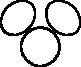
\includegraphics[width=0.09\textwidth]{%
gesamttex/edit_VIII,3/images/LH_37_05_094-095_d_8_095v.pdf%
}\hfill} 
\vspace{0.5em}
\centerline{\hspace*{10mm}\hfill%
\lbrack\textit{Fig.~7}\rbrack\hfill\hspace*{5mm}\lbrack\textit{Fig.~8}\rbrack%
\hfill}
% \newpage%
\vspace{1em}
%
\pstart
%
Suffecerit nos in summa pro
%
\edtext{velocitatibus\protect\index{Sachverzeichnis}{velocitas} ipsorum}{%
\lemma{velocitatibus}%
\Bfootnote{%
\textit{(1)}~ipsarum %
\textit{(2)}~ipsorum~\textit{L}}}
%
corporum post ictum\protect\index{Sachverzeichnis}{ictus}
%
\edtext{definiendis Theoremata non contemnenda%
\protect\index{Sachverzeichnis}{theorema non contemnendum} invenisse, ex quibus etiam}{%
\lemma{definiendis}%
\Bfootnote{%
\textit{(1)}~Theorema non contemnendum %
\textit{(2)}~Theoremata non contemnenda %
\textit{(a)}~adhibuisse %
\textit{(b)}~invenisse, %
\textit{(aa)}~quae etiam ex %
\textit{(bb)}~ex quibus etiam~\textit{L}}}
%
 manifestum est \textit{y} evanescere et \textit{x} fieri $=l$ eo casu quo anguli componentium directionum sint recti.%
\protect\index{Sachverzeichnis}{angulus rectus}  
%
Supposuit autem demonstratio nostra  
%
directiones \textit{{\scriptsize1}B{\scriptsize2}B}, \textit{{\scriptsize1}C{\scriptsize2}C} esse  
%
in rectis \textit{M{\scriptsize2}A}, \textit{L{\scriptsize2}A}
%
\edtext{continuatis, quia}{%
\lemma{continuatis,}%
\Bfootnote{%
\textit{(1)}~quod pro certo habendum \textbar\ est, \textit{streicht Hrsg.}~\textbar\ %
\textit{(2)}~quia~\textit{L}}}
%
si quodlibet
%
\edtext{corpus \textit{B}}{%
\lemma{corpus}%
\Bfootnote{%
\textit{(1)}~separatim %
\textit{(2)}~\textit{B}~\textit{L}}}
%
vel \textit{C} separatim
%
\edtext{excipiat ita}{%
\lemma{excipiat}%
\Bfootnote{%
\textit{(1)}~\textit{A} ita \textit{(2)}~ita~\textit{L}}}
%
 impelletur, nunc autem cum ambo adsint, in hoc quidem alterum
%
\edtext{alteri non videtur derogare. Verum nunc re melius expensa dubitare incipio, et vereor, %
ne compressiones\protect\index{Sachverzeichnis}{compressio} duplices}{%
\lemma{alteri}%
\Bfootnote{%
\textit{(1)}~nil derogat. Nisi %
\textit{(a)}~quis %
\textit{(b)}~forte vereri velimus %
\textit{(2)}~non videtur \lbrack...\rbrack\ vereor, ne %
\textit{(a)}~compressio %
\textit{(aa)}~duplex %
\textit{(bb)}~duplex %
\textit{(b)}~compressiones duplices~\textit{L}}}
%
 globi\protect\index{Sachverzeichnis}{globus} incurrentis, se mutuo alterent, ita ut angulus \textit{B.{\scriptsize2}A.C}  
%
fiat multo minor quam angulus \textit{L{\scriptsize2}AM}, quando hic non est rectus. Et quid si hic  
%
quoque locum haberet,
%
\edtext{quod in duorum}{%
\lemma{quod in}%
\Bfootnote{%
\textit{(1)}~simplicibus corporibus %
\textit{(2)}~duorum~\textit{L}}}
%
tantum corporum concursu,\protect\index{Sachverzeichnis}{concursus}
%
\edtext{concursu, et in casu}{%
\lemma{concursu, et}%
\Bfootnote{%
\textit{(1)}~ut %
\textit{(2)}~in casu~\textit{L}}}
%
trium
%
\edtext{cum angulus}{%
\lemma{cum}%
\Bfootnote{%
\textit{(1)}~directio %
\textit{(2)}~angulus~\textit{L}}}
%
 \textit{L.{\scriptsize2}A.M} est rectus,%
\protect\index{Sachverzeichnis}{angulus rectus} ut scilicet sumatur ${\scriptstyle \textit{3}}AH={\scriptstyle \textit{1}}A.G$ 
%
et $HD=G{\scriptstyle \textit{2}}A$ vel \textit{G{\scriptsize2}B}
%
\edtext{vel \textit{G{\scriptsize2}C}, adeoque}{%
\lemma{vel \textit{G{\scriptsize2}C},}%
\Bfootnote{%
\textit{(1)}~seu %
\textit{(2)}~adeoque~\textit{L}}}
%
ut \textit{A} tantum recedat a centro gravitatis corporum \textit{A} quantum ad ipsa accessit.  
%
Quo posito etiam \textit{A} repelletur, cum angulus est obliquus,%
\protect\index{Sachverzeichnis}{angulus obliquus}
%
quod ipsum etiam ex eo concludo, quod \textit{A} repellitur si corpora \textit{B} et \textit{C} 
%
ita sint sita, ut angulus \textit{B{\scriptsize2}AC} sit summe acutus,%
\protect\index{Sachverzeichnis}{angulus summe acutus} quod 
%
\edtext{fit si corpora \textit{B} et \textit{C} quasi}{%
\lemma{fit si corpora \textit{B} et \textit{C}}%
\Bfootnote{%
\textit{(1)}~sint tam parva, ut quasi co %
\textit{(2)}~quasi~\textit{L}}}
%
coincidant in eandem rectam, (quem in usum debent satis esse parva) quo
%
\edtext{casu ponenda}{%
\lemma{casu}%
\Bfootnote{%
\textit{(1)}~constat %
\textit{(2)}~ponenda~\textit{L}}}
%
 sunt quasi unum corpus, et tunc constat si \textit{A} incurrat in quiescens sui duplum non pergere sed
%
\edtext{repelli. Contra}{%
\lemma{repelli.}%
\Bfootnote{%
\textit{(1)}~Similiter %
\textit{(2)}~Contra~\textit{L}}}
%
si angulus \textit{B{\scriptsize2}AC} sit summe obtusus,%
\protect\index{Sachverzeichnis}{angulus summe obtusus} seu si \textit{{\scriptsize2}B}, \textit{{\scriptsize2}A},  
%
\textit{{\scriptsize2}C} cadant in eandem rectam, tunc nullus fit ictus, sed \textit{A} pergit. Itaque quo magis acutus%
\protect\index{Sachverzeichnis}{angulus acutus}  
%
angulus eo magis repellitur \textit{A}, quo magis obtusus,%
\protect\index{Sachverzeichnis}{angulus obtusus} eo magis progreditur \textit{A}; denique si sit rectus angulus,%
\protect\index{Sachverzeichnis}{angulus rectus}  
%
tunc \textit{A} nec progreditur  nec repellitur sed quiescit. Idem etiam patet ex valore ipsius \textit{y} quem ex posita  
%
angulus retentione duximus nam in casu anguli recti $2ll-aa=0$ et $y=0$ seu \textit{A}
%
\edtext{quiescit, in casu anguli obtusi\protect\index{Sachverzeichnis}{angulus obtusus}}{%
\lemma{quiescit, in casu anguli}%
\Bfootnote{%
\textit{(1)}~acuti %
\textit{(2)}~obtusi~\textit{L}}}
%
 $2ll$ majus \textit{aa}, et \textit{A} progreditur\lbrack,\rbrack\ in casu denique anguli acuti%
\protect\index{Sachverzeichnis}{angulus acutus} \textit{ll}  
%
est minus \textit{aa}, ergo \textit{y} fit quantitas negativa seu \textit{A} repellitur. Sed haec ducta
%
\edtext{ex falsa}{%
\lemma{ex}%
\Bfootnote{%
\textit{(1)}~calculo \textit{(2)}~falsa~\textit{L}}}
%
 hypothesi anguli ejusdem
%
\edtext{manentis. Saltem certum est in angulo}{%
\lemma{manentis.}%
\Bfootnote{%
\textit{(1)}~\textlangle\textendash \textendash \textendash \textendash \textendash\textrangle ne in angulo quidem  %
\textit{(2)}~Saltem certum est %
\textit{(3)}~Saltem certum est in angulo~\textit{L}}}
%
recto
\edtext{\textit{B{\scriptsize2}AC},}{%
\lemma{recto}%
\Bfootnote{%
\textit{(1)}~directi %
\textit{(2)}~directi %
\textit{(3)}~\textit{B{\scriptsize2}AC},~\textit{L}}}
%
tam
%
\edtext{succedere ut simul}{%
\lemma{succedere}%
\Bfootnote{%
\textit{(1)}~\textlangle\textendash\textrangle\ simul %
\textit{(2)}~\textlangle\textendash\textrangle\ %
\textit{(3)}~ut %
\textit{(a)}~fiet %
\textit{(b)}~simul~\textit{L}}}
%
potentiae,\protect\index{Sachverzeichnis}{potentia} via centri\protect\index{Sachverzeichnis}{via centri gravitatis} %
et angulus directionum%
\protect\index{Sachverzeichnis}{angulus directionum} serventur. Inspiciatur figura, si angulus \textit{LAM} rectus  
%
et servatur in excipie\textlangle ndo\textrangle\ \textlangle\textendash\ \textendash\textrangle\ 
%
\textit{BAC} sit angulus rectus utique ut servetur potentia\protect\index{Sachverzeichnis}{potentia} erunt  
%
\textit{{\scriptsize1}B{\scriptsize2}B}, \textit{{\scriptsize1}C{\scriptsize2}C}, ipsis \textit{LA}, \textit{MA} aequales.
%
Porro centrum Gravitatis\protect\index{Sachverzeichnis}{centrum gravitatis} %
in statu \textit{{\scriptsize1}A}.\textit{{\scriptsize1}B}.\textit{{\scriptsize1}C} est \textit{G}, ita ut sit
%
\edtext{$G{\scriptstyle \textit{2}}A=$ triens}{%
\lemma{$G{\scriptstyle \textit{2}}A=$}%
\Bfootnote{%
\textit{(1)}~${\scriptstyle\textit{1}}A{\scriptstyle\textit{2}}A:3$ %
\textit{(2)}~triens~\textit{L}}}
%
de \textit{{\scriptsize1}A{\scriptsize2}A}, centrum autem gr.\
%
aequabiliter progreditur ergo fit ${\scriptstyle \textit{2}}AH=G{\scriptstyle \textit{2}}A$, seu \textit{GH} dupla  
%
\textit{G{\scriptsize2}A}. Ergo ob \textit{D} centrum gr.\protect\index{Sachverzeichnis}{centrum gravitatis} ipsorum  
%
\textit{{\scriptsize2}B} et \textit{{\scriptsize2}C} erit \textit{HD} dimidia \textit{{\scriptsize2}AH}. Ergo tota  
%
\textlangle\textit{\scriptsize2}\textrangle\textit{AD} debet esse dimidia ipsius \textit{{\scriptsize1}A{\scriptsize2}A} quod et
%
\edtext{succedit ni velimus}{%
\lemma{succedit}%
\Bfootnote{%
\textit{(1)}~illud vero non evenit \textit{(2)}~ni velimus~\textit{L}}}
%
 ut sit $H{\scriptstyle \textit{3}}A=G{\scriptstyle \textit{1}}A$. Ita enim et repelleretur, ergo 
%
\textit{{\scriptsize1}B{\scriptsize2}B}, \textit{{\scriptsize1}C{\scriptsize2}C} fierent minores quam \textit{LA}  
%
et quia tunc \textit{HC} fieret aequ.\ \textit{H{\scriptsize2}A}, utique angulum \textit{B{\scriptsize2}AC}  
%
eveniret fieri acutum.%
\protect\index{Sachverzeichnis}{angulus acutus} 
\pend
\count\Afootins=1200%
\count\Bfootins=1200%
\count\Cfootins=1200